
\documentclass[]{article}

\usepackage[italian]{babel}
\usepackage[margin=20mm, footskip = 20pt]{geometry}
\usepackage{array}
\usepackage{tabularx}
\usepackage{graphicx}
\usepackage{subfiles}
\usepackage{hyperref}
\usepackage{nameref}
\usepackage{titlesec}
\usepackage{longtable}
\usepackage[table]{xcolor}
\usepackage{titling}
\usepackage{lastpage}
\usepackage{ifthen}
\usepackage{calc}
\usepackage{soulutf8}
\usepackage{contour}
\usepackage{float}
\usepackage{fancyhdr}
\usepackage{multirow}
\usepackage{pgfgantt}
\usepackage{lscape}

\newcommand{\hr}{\par\vspace{-.1\ht\strutbox}\noindent\hrulefill\par}

\graphicspath{ {./}
	{./commons/res}
}

%--------------------------------------------------
% Comandi per inserire contenuto del documento
%--------------------------------------------------
\makeatletter

\newcommand\appendToGraphicsPath[1]{%
	\g@addto@macro\Ginput@path{{#1}}%
}

\newcommand{\setTitle}[1]{%
	\newcommand{\@phTitle}{#1}%
}
\newcommand{\phTitle}{\@phTitle}

\newcommand{\setDate}[1]{%
	\newcommand{\@phDate}{#1}%
}
\newcommand{\phDate}{\@phDate}

\newcommand{\setUso}[1]{%
	\newcommand{\@uso}{#1}%
}
\newcommand{\uso}{\@uso}

\newcommand{\setVersione}[1]{%
	\newcommand{\@versione}{#1}%
}
\newcommand{\versione}{\@versione}

\newcommand{\disabilitaVersione}{%
	\renewcommand{\setVersione}[1]{}%
	\renewcommand{\versione}{DISABILITATA}
}

\newcommand{\setResponsabile}[1]{%
	\newcommand{\@responsabile}{#1}%
}
\newcommand{\responsabile}{\@responsabile}

\newcommand{\setRedattori}[1]{%
	\newcommand{\@redattori}{#1}%
}
\newcommand{\redattori}{\@redattori}

\newcommand{\setVerificatori}[1]{%
	\newcommand{\@verificatori}{#1}%
}
\newcommand{\verificatori}{\@verificatori}

\newcommand{\setModifiche}[1]{%
	\newcommand{\@modifiche}{#1}%
}
\newcommand{\modifiche}{\@modifiche}

\makeatother 

%--------------------------------------------------
% Comandi per i documenti esterni e il glossario
%--------------------------------------------------

\newcommand{\dext}[1]{\textsc{#1\textsubscript{\textit{D}}}}

\newcommand{\glock}[1]{\textsc{#1\textsubscript{\textit{G}}}}

%--------------------------------------------------
% Comandi per impostare sottotitoli di quarto e quinto livello
%--------------------------------------------------

\setcounter{secnumdepth}{4}
\setcounter{tocdepth}{4}

\titleformat{\paragraph}
{\normalfont\normalsize\bfseries}{\theparagraph}{1em}{}
\titlespacing*{\paragraph}{0pt}{2.25ex plus 1ex minus .2ex}{1.5ex plus .2ex}

\titleformat{\subparagraph}
{\normalfont\normalsize\bfseries}{\thesubparagraph}{1em}{}
\titlespacing*{\subparagraph}{0pt}{1.75ex plus 1ex minus .2ex}{.75ex plus .1ex}

\appendToGraphicsPath{../../commons/res/}
\usepackage[export]{adjustbox}


%------------------------------
%
% COMANDI DI CONFIGURAZIONE
%
%------------------------------

\setTitle{Piano di Progetto}

\setVersione{4.0.0}

\setDate{25-07-2021}

\setResponsabile{Alessandro Chimetto}

\setRedattori{
	Alessandro Chimetto \\&
	Alessandro Dindinelli\\&
	Giacomo Bulbarelli\\&
	Lucia Fenu \\&
	Matteo Alba \\&
	Paolo Scanferlato\\&
  	Valton Tahiraj
}

\setVerificatori{
    Alessandro Chimetto \\&
	Alessandro Dindinelli\\&
	Giacomo Bulbarelli\\&
	Lucia Fenu\\&
	Paolo Scanferlato\\&
	Valton Tahiraj
}

\setUso{Esterno}

\setModifiche{
	4.0.0 & Giacomo Bulbarelli & Verificatore & Approvazione documento & 22-08-2021\\
	3.2.0 & Lucia Fenu & Amministratore & Aggiunto fine dei periodi nella sezione riscontro rischi & 21-08-2021\\
	3.1.0 & Lucia Fenu, \hspace{1cm} Paolo Scanferlato & Amministratore, Verificatore & 10-08-2021, 20-08-2021 & Aggiornato Preventivo e Pianificazione, verificato\\
	3.0.0 & Alessandro Chimetto & Responsabile & 18-07-2021 & Approvazione documento v3.0.0\\
	2.1.0 &	Lucia Fenu, \hspace{1cm} Valton Tahiraj  	& Amministratore, Verificatore   &17-07-2021  & Aggiornati e verificati consuntivo,preventivo e pianificazione\\
    2.0.0 & Matteo Alba           & Responsabile   & 14-03-2021 & Approvazione documento v2.0.0 \\
    1.4.0 & Lucia Fenu, Alessandro Chimetto& Amministratore, Verificatore   & 14-03-2021 & Aggiunta e verificato § Consuntivo\\
	1.3.0 & Lucia Fenu, Giacomo Bulbarelli& Amministratore, Verificatore   & 14-03-2021 & Aggiunta e verificato § Pianificazione\\
	1.2.0 & Lucia Fenu, Paolo Scanferlato     & Amministratore, Verificatore   & 14-03-2021 & Aggiunta e verificato § Preventivo\\
    1.1.0 & Alessandro Dindinelli, Alessandro Chimetto   & Amministratore, Verificatore   & 13-03-2021 & Aggiunta e verificato § Riscontro rischi\\
	1.0.0 & Lucia Fenu			  & Responsabile   & 10-01-2021 & Approvazione documento v1.0.0\\
	0.8.0 & Giacomo Bulbarelli, Lucia Fenu 			  & Amministratore, Verificatore   & 08-01-2021 & Aggiunta e verifica § Rischi\\
	0.7.0 & Paolo Scanferato, Valton Tahiraj  	  & Amministratore, Verificatore   & 06-01-2021 & Aggiunta e verifica correzioni § Preventivo tabelle e grafici\\
	0.6.0 & Lucia Fenu, Valton Tahiraj        & Amministratore, Verificatore   & 06-01-2021 & Aggiunta e verificata § Consuntivo \\
	0.5.0 & Matteo Alba, Valton Tahiraj        & Amministratore, Verificatore   & 05-01-2021 & Aggiunta e verificata § Pianificazione \\
    0.4.0 & Giacomo Bulbarelli, Paolo Scanferlato     & Amministratore, Verificatore   & 04-01-2021 & Aggiunta e verificato § Analisi dei rischi \\
	0.3.0 & Valton Tahiraj, Alessandro Dindinelli & Amministratore, Verificatore   & 30-12-2020 & Aggiunta e verificato § Organigramma \\
	0.2.0 & Alessandro Chimetto, Alessandro Dindinelli & Amministratore, Verificatore   & 27-12-2020 & Aggiunta e verificato § Modello di ciclo di Vita \\
    0.1.0 & Alessandro Dindinelli, Alessandro Chimetto   & Amministratore, Verificatore   & 26-12-2020 & Aggiunta e verificata § Introduzione \\
    0.0.1 & Alessandro Dindinelli, Alessandro Chimetto   & Amministratore, Verificatore   & 24-12-2020 & Stesura e verifica primo scheletro del documento 
}

\begin{document}

	% Direttive per la creazione del titolo tramite comando maketitle
\title{\huge \textsc{\phTitle{}} \\
	\vspace{11pt} \large \textsc{\phDate{}}}

\author{} % Non toccare
\date{} % Non toccare

%--------------------
% Frontespizio
%--------------------

% Logo del gruppo
\begin{figure}[t!]
	\centering
	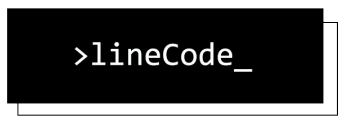
\includegraphics[width=20em]{lclong}
\end{figure}

% Titolo / Nome
\maketitle
\thispagestyle{empty}

% Dati specifici sul doc in forma tabulare
\begin{table}[ht]
	\begin{center}
		\label{tab:Dati sul documento}
		\begin{tabular}{r|l}
			\multicolumn{2}{c}{ \textsc{Dati sul documento} } \\
			\hline
			\textbf{Versione} & \versione{} \\
			\textbf{Uso} & \uso{}  \\
			\textbf{Redattori} & \redattori{} \\
			\textbf{Verificatori} & \verificatori{} \\
			\textbf{Responsabile} & \responsabile{} \\
			\textbf{Destinatari} & lineCode \\
								& prof.\ Vardanega Tullio \\		
								& prof.\ Cardin Riccardo \\
			\ifthenelse{\equal{\uso}{Esterno}}{
								& Sanmarco Informatica
			}{} \\
		\end{tabular}
	\end{center}
\end{table}

\newpage

\renewcommand{\arraystretch}{2} % allarga le righe con dello spazio sotto e sopra
\begin{longtable}[H]{>{\centering\bfseries}m{2cm} >{\centering}m{3.5cm} >{\centering}m{2.5cm} >{\centering}m{3cm} >{\centering\arraybackslash}m{5cm}}
	\rowcolor{lightgray}
	{\textbf{Versione}} & {\textbf{Nominativo}} & {\textbf{Ruolo}} & {\textbf{Data}} & {\textbf{Descrizione}}  \\
	\endfirsthead%
	\rowcolor{lightgray}
	{\textbf{Versione}} & {\textbf{Nominativo}}  & {\textbf{Ruolo}} & {\textbf{Data}} & {\textbf{Descrizione}}  \\
	\endhead%
	\modifiche{}%
\end{longtable}
	\newpage
	\tableofcontents
	\newpage
	\listoffigures
	\listoftables
	\newpage

	%--------------------------------
	%
	% IL CONTENUTO INIZIA DA QUI
	%
	%--------------------------------

	\section{Introduzione}
	\subsection{Scopo del documento}
Il documento ha lo scopo di definire le guidelines del way of working adottato dal team lineCode. Le attività presenti in questo documento sono redatte da processi contenuti nello standard ISO/IEC 12207:1995. Risulta quindi necessario che tutti i membri del gruppo prendano visione di questo documento ai fini di coesione e uniformità all'interno del progetto.

\subsection{Scopo del prodotto}
Il \glock{capitolato} C5 ha come obbiettivo la realizzazione di un applicativo \glock{Real-Time} in grado di guidare delle unità dotate di mobilità autonoma in ambienti specifici, partendo dal presupposto che queste si muovano in ambienti in cui sono presenti altre unità (autonome o meno).

\subsection{Glossario e documenti esterni}
In supporto alla documentazione viene fornito un glossario per chiarire, con una definizione, eventuali termini specifici contenuti in questo documento.
Saranno adottati quindi questi due simboli a pedice:
\begin{itemize}
	\item \textit{D} se indicano un documento specifico;
	\item \textit{G} se incluse nel \dext{glossario}.
\end{itemize}

\subsection{Riferimenti}
	\subsubsection{Riferimenti normativi}
	\begin{itemize}
		\item \textbf{{C5 - PORTACS}}: \url{https://www.math.unipd.it/~tullio/IS-1/2020/Progetto/C5.pdf};
        \item \textbf{Oracle Java Code Conventions}: \url{https://www.oracle.com/technetwork/java/codeconventions-150003.pdf};
        \item \textbf{Angular coding style guide}: \url{https://angular.io/guide/styleguide}.
	\end{itemize}
	\subsubsection{Riferimenti informativi}
	\begin{itemize}
		\item \textbf{ISO/IEC 12207:1995}: \url{https://www.math.unipd.it/~tullio/IS-1/2009/Approfondimenti/ISO_12207-1995.pdf};
		\item \textbf{Gitflow}: \url{http://nvie.com/posts/a-successful-git-branching-model/};
		\item \textbf{Documentazione Zapier}: \url{https://zapier.com/help};
		\item \textbf{Documentazione act}: \url{https://github.com/nektos/act/blob/master/README.md};
		\item \textbf{Studio di Fattibilità}: \dext{Studio di Fattibilità v1.0.0};
		\item \textbf{Piano di Qualifica}: \dext{Piano di Qualifica v2.0.0};
		\item \textbf{Piano di Progetto}: \dext{Piano di Progetto v2.0.0}.
	\end{itemize}
	\newpage

	\section{Analisi dei rischi}
		Al fine di garantire il successo dell'attività di progetto, risulta necessario definire un piano per la gestione dei rischi. \\
	Nello specifico, tale piano è composto da quattro attività:
	\begin{enumerate}
		\item \textbf{Identificazione dei rischi}: attività che si pone l'obiettivo di identificare e definire i rischi che possono insorgere nel corso dell'attività di progetto. In particolare, essa si propone di dare un identificativo e una descrizione ai rischi che emergono durante l'attività.
		\item \textbf{Analisi dei rischi}: attività di analisi che consiste nello studio di ciascuno dei rischi identificati, al fine di evidenziare:
		\begin{itemize}
			\item probabilità di occorrenza;
			\item fattore di rischio;
			\item conseguenze che il manifestarsi del rischio potrebbe avere.
		\end{itemize}
		\item \textbf{Pianificazione di controllo e mitigazione}: attività che si propone di:
			\begin{itemize}
				\item stabilire le modalità attraverso cui prevenire il verificarsi di un rischio;
				\item stabilire le modalità attraverso cui reagire al verificarsi di un rischio.
			\end{itemize}
			I prodotti di questa attività sono dunque:
			\begin{itemize}
				\item metodi di controllo dei rischi;
				\item piano di contingenza.
			\end{itemize}
		\item \textbf{Monitoraggio dei rischi}: attività che si propone di monitorare i rischi al fine di prevenirli, e di permettere una reazione tempestiva nel caso in cui questi si verifichino. Il prodotto di tale attività sono delle metodologie di rilevamento di rischi.
	\end{enumerate}
	
	I rischi rilevati nel contesto specifico dell'attività progettuale proposta sono riassumibili nelle seguenti categorie:
	\begin{enumerate}
		\item rischi legati alle dinamiche di gruppo;
		\item rischi legati all'organizzazione del lavoro;
		\item rischi legati ai requisiti;
		\item rischi legati ai mezzi tecnologici.
	\end{enumerate}

\subsection{Rischi legati alle dinamiche di gruppo}
	\subsubsection{Inesperienza del gruppo}	
	\begin{enumerate}
		\item \textbf{Descrizione e conseguenze}: nessun membro del gruppo ha mai affrontato prima un progetto come questo dal punto di vista dell'impegno richiesto, del tempo richiesto, delle conoscenze da acquisire e del numero di persone con cui è necessario coordinarsi. Ciò può portare a conseguenze non desiderabili, quali ritardi e difficoltà nel sincronizzare il lavoro;
		\item \textbf{Probabilità di occorrenza}: alta;
		\item \textbf{Fattore di rischio}: alto;
		\item \textbf{Rilevamento}: ciascun membro che dovesse incontrare difficoltà provvederà a comunicarlo immediatamente al Responsabile. Se un qualsiasi compito tarda ad essere ultimato, è onere del Responsabile informarsi sullo stato dei lavori. 
		\item \textbf{Controllo}: il Responsabile aiuterà i membri che incontrano difficoltà attraverso delle attività di auto-miglioramento.
		\item \textbf{Piano di contingenza}: il membro in difficoltà consulterà il Responsabile, il quale provvederà a riportare la problematica al gruppo chiedendo aiuto ad un altro componente che andrà a fornire supporto nell'analisi delle criticità incontrate e nella risoluzione del problema affrontato, accelerando il completamento del lavoro.
	\end{enumerate}
	
	\subsubsection{Indisponibilità}
	\begin{enumerate}
		\item \textbf{Descrizione e conseguenze}: tutti i membri del gruppo sono studenti a tempo pieno. Impegni Universitari e personali potrebbero portare all'indisponibilità momentanea di alcuni membri, portando a ritardi e a complicazioni del lavoro da svolgere; 
		\item \textbf{Probabilità di occorrenza}: media;
		\item \textbf{Fattore di rischio}: medio;
		\item \textbf{Rilevamento}: qualora un membro risultasse indisponibile, provvederà a comunicarlo tempestivamente al Responsabile;
		\item \textbf{Controllo}: il Responsabile provvederà a informarsi della disponibilità dei singoli membri e a coordinare il gruppo di conseguenza;
		\item \textbf{Piano di contingenza}: nel caso in cui un membro risultasse indisponibile, il Responsabile provvederà a comunicarlo al gruppo e a coordinare la nuove distribuzione del lavoro sugli altri membri disponibili.
	\end{enumerate}
	
	\subsubsection{Contrasti interni}
	\begin{enumerate}
		\item \textbf{Descrizione e conseguenze}: i membri del gruppo non si conoscevano prima di intraprendere questo progetto. Il numero elevato di componenti del gruppo unito alla scarsa conoscenza che i membri hanno reciprocamente sia a livello personale che lavorativo, potrebbero portare all'insorgere contrasti interni al gruppo con conseguente deterioramento del clima lavorativo;
		\item \textbf{Probabilità di occorrenza}: bassa;
		\item \textbf{Fattore di rischio}: molto alto;
		\item \textbf{Rilevamento}: il Responsabile monitorerà costantemente le interazioni tra i membri e li inviterà a informarlo nel caso in cui vi siano delle difficoltà;
		\item \textbf{Controllo}: il Responsabile andrà a moderare gli incontri tra i membri e avrà l'onere di assicurare un ambiente di lavoro sano per tutti. 
		\item \textbf{Piano di contingenza}: nel caso in cui vi siano dei conflitti interni tra i membri, il Responsabile si proporrà di moderare un incontro tra i membri in conflitto (escludendo eventualmente i membri non interessati) e fungerà da mediatore nel corso del suddetto incontro.
	\end{enumerate}
	
\subsection{Rischi legati all'organizzazione del lavoro}
	\subsubsection{Pianificazione delle attività}
	\begin{enumerate}
		\item \textbf{Descrizione e conseguenze}: ciascuna attività ha un costo in termini di tempo. Un errata pianificazione delle stesse potrebbe portare a rallentamenti e compromettere lo sviluppo; 
		\item \textbf{Probabilità di occorrenza}: media;
		\item \textbf{Fattore di rischio}: alto;
		\item \textbf{Rilevamento}: nel caso in cui un membro non sia in grado di svolgere gli incarichi assegnatigli nei tempi previsti, provvederà a comunicarlo tempestivamente al Responsabile;		
		\item \textbf{Controllo}: ad ogni incontro ciascun membro notificherà il Responsabile e gli altri membri circa lo stato dei propri lavori e si provvederà a fare un confronto tra i tempi di esecuzione del lavoro previsti e quelli effettivi; 
		\item \textbf{Piano di contingenza}: il Responsabile provvederà a coordinare il gruppo per redistribuire il lavoro in eccesso e moderare la nuova pianificazione dei lavori.
	\end{enumerate}
	
\subsection{Rischi legati ai requisiti}
	\subsubsection{Analisi dei rischi incompleta o incorretta}
	\begin{enumerate}
		\item \textbf{Descrizione e conseguenze}: data l'inesperienza del gruppo è possibile che il prodotto dell'analisi dei requisiti sia incompleto o incorretto. Tale scenario porterebbe a notevoli rallentamenti dei lavori;
		\item \textbf{Probabilità di occorrenza}: media;
		\item \textbf{Fattore di rischio}: medio;
		\item \textbf{Rilevamento}: in caso di dubbi o incertezze in sede di analisi, ciascuno dei membri è tenuto a comunicarlo al Responsabile e agli altri membri del gruppo;		
		\item \textbf{Controllo}: l'analisi dei requisiti verrà periodicamente rivista e controllata in fase di redazione al fine di migliorarla e raffinarla continuativamente.
		\item \textbf{Piano di contingenza}: nel caso in cui vengano evidenziate imprecisioni o inesattezze da parte del proponente in sede di revisione, il gruppo provvederà a correggere gli errori nel minor tempo possibile.
	\end{enumerate}
	
	\subsubsection{Modifica dei requisiti}
	\begin{enumerate}
		\item \textbf{Descrizione e conseguenze}: è possibile che il proponente SanMarco Informatica decida di aggiungere dei requisiti in corso d'opera, portando alla necessità di modificare l'analisi dei requisiti precedentemente svolta; 
		\item \textbf{Probabilità di occorrenza}: bassa;
		\item \textbf{Fattore di rischio}: medio;
		\item \textbf{Rilevamento}: il gruppo si propone di contattare in maniera cadenzata il proponente durante lo sviluppo per mantenere sincronizzate le due parti;
		\item \textbf{Controllo}: il gruppo si propone di tracciare quanto viene deciso e discusso con il proponente dopo ogni incontro;
		\item \textbf{Piano di contingenza}: nel caso in cui sia necessario modificare dei requisiti, il gruppo provvederà a svolgere le attività di analisi e correzione della documentazione nel minor tempo possibile.
	\end{enumerate}	
	
\subsection{Rischi legati ai mezzi tecnologici}
	\subsubsection{Tecnologie da usare}		
	\begin{enumerate}
		\item \textbf{Descrizione e conseguenze}: le tecnologie da usare sono varie e spesso non conosciute da tutti i membri del gruppo. I tempi di apprendimento di tali tecnologie potrebbero portare a ritardi e difficoltà nello svolgimento del progetto;
		\item \textbf{Probabilità di occorrenza}: alta;
		\item \textbf{Fattore di rischio}: alto;
		\item \textbf{Rilevamento}: i membri che hanno delle difficoltà a interfacciarsi con una specifica tecnologia provvederanno a comunicarlo tempestivamente al responsabile del gruppo;
		\item \textbf{Controllo}: il Responsabile provvederà a coordinare i membri rispetto alle conoscenze necessarie per poter utilizzare una determinata tecnologia;  
		\item \textbf{Piano di contingenza}: al rilevamento di una difficoltà nell'interfacciarsi con una specifica tecnologia, il Responsabile provvederà a indirizzare i componenti verso le risorse utili e, qualora fosse necessario, coordinare una riunione per compensare e correggere le criticità che i membri presentano.
	\end{enumerate}	
	
	\subsubsection{Problemi Hardware}
	\begin{enumerate}
		\item \textbf{Descrizione e conseguenze}: ciascuno dei componenti lavora su macchine private. Un guasto a una di queste, potrebbe portare a rallentamenti del lavoro o perdita di dati;
		\item \textbf{Probabilità di occorrenza}: media;
		\item \textbf{Fattore di rischio}: basso;
		\item \textbf{Rilevamento}: ciascun membro che presenta dei problemi con la propria macchina provvede a comunicarlo al Responsabile;		
		\item \textbf{Controllo}: ciascun membro cerca, per quanto possibile, di avere cura della propria attrezzatura.
		\item \textbf{Piano di contingenza}: in caso di problematiche specifiche i membri sono tenuti a comunicarlo tempestivamente per permettere di organizzare il lavoro di conseguenza. Provvederanno poi a sostituire le componenti corrotte. 
	\end{enumerate}
	
	\subsubsection{Problemi Software}
	\begin{enumerate}
		\item \textbf{Descrizione e conseguenze}: il gruppo si appoggia a piattaforme online per la condivisione dei dati e per la comunicazione tra i membri. Data anche l'attuale situazione sanitaria che obbliga a lavorare per via telematica, un malfunzionamento di tali piattaforme potrebbe compromettere la comunicazione e il lavoro del gruppo;
		\item \textbf{Probabilità di occorrenza}: bassa;
		\item \textbf{Fattore di rischio}: alto;
		\item \textbf{Rilevamento}: i membri del gruppo monitoreranno le piattaforme utilizzate;
		\item \textbf{Controllo}: non attuabile, non si ha controllo sulle piattaforme esterne; 
		\item \textbf{Piano di contingenza}: non pianificabile a priori. Si applica un azione reattiva e correttiva nel caso dovessero verificarsi malfunzionamenti.
	\end{enumerate}		

	\newpage

	\section{Modello di sviluppo}
	Il modello di ciclo di vita utilizzato è fortemente ispirato al modello
incrementale. Lo sviluppo avviene per incrementi dove ogni incremento rilascia parte delle funzionalità richieste.
\\\\
I requisiti vengono inizialmente classificati in base alla loro priorità e viene
creata un'architettura che permetta la successiva aggiunta di molteplici
incrementi. Ciò permette di sviluppare fin da subito un insieme di funzionalità
fondamentali e stabili. Segue il soddisfacimento di requisiti meno importanti e
meno chiari che, nel tempo, riescono a stabilizzarsi ed integrarsi con quanto già
realizzato.
\\\\
Il modello presenta i seguenti vantaggi:
\begin{itemize}
    \item ogni incremento può essere verificato prima dell'integrazione rendendo la verifica economica perché la parte già realizzata è stata precedentemente verificata;
    \item ogni incremento rende disponibili nuove funzionalità e chiarisce i requisiti per incrementi successivi;
    \item ad ogni incremento è possibile ricevere un feedback da committente o proponente;
    \item una volta realizzato ed integrato, ogni incremento riduce la probabilità che il progetto fallisca.
\end{itemize}

\noindent
Nonostante il modello incrementale non preveda che gli incrementi già realizzati
possano subire successivi interventi correttivi o di raffinamento (come invece
accadrebbe in un modello iterativo) e, vista la mancanza di sufficiente esperienza
in progetti software di tali dimensioni; il gruppo si riserva il diritto di
effettuare iterazioni potenzialmente distruttive sul prodotto già realizzato.
Questa pratica, che comunque viene considerata non desiderabile, verrà messa in
atto solo dopo un eventuale feedback negativo da parte del proponente durante il
confronto che segue la realizzazione di un iterazione.

	\newpage

	\section{Pianificazione}
	Per poter assicurare una conduzione e uno sviluppo del progetto che soddisfino le scadenze riportate nella sezione xxx, il gruppo ha deciso di ripartire il lasso di tempo che va dalla sua formazione fino alla revisione di accettazione nelle seguenti cinque attività:
	
	\begin{itemize}
		\item Analisi dei requisiti
		\item Consolidamento dei requisiti
		\item Progettazione della technology baseline
		\item Progettazione di dettaglio e codifica
		\item Validazione e collaudo
	\end{itemize}
	
	Ogni attività verrà poi frammentata in altri sottoperiodi, in ognuno dei quali verrà associata una \glock{Milestone},
	riferita alla data di fine periodo, per il completamento delle singole attività previste al suo interno.
	In intervallo di tempo vengono quindi inserite più attività, le quali possono essere svolte sia sequenzialmente,
	sia con un certo grado di parallelismo, in base alle dipendenze che sussistono tra di loro.
	
	\subsection{Analisi dei Requisiti}
	L’attività di analisi dei requisiti ha inizio il giorno 31-10-2021, successivamente alla formazione dei
	gruppi, ed è suddivisa in cinque periodi, con termine fissato per il giorno 11-01-2021, giorno di consegna dei documenti in ingresso alla revisione dei requisiti.
	
	\subsection{Ruoli attivi}
	Durante questa attività è necessaria la presenza dei seguenti ruoli:
	\begin{itemize}
		\item responsabile;
		\item amministratore;
		\item analista;
		\item verificatore;
	\end{itemize}

	\subsection{Periodi}
	L’attività di analisi dei requisiti è stata suddivisa nei seguenti cinque periodi:
	
	\subsubsection{Primo periodo dal 31-10-2021 al 05-12-2021}
	\begin{itemize}
	\item \textbf{Analisi dei capitolati}: studio individuale dei capitolati e discussione interna al gruppo dei pregi e svantaggi individuati da ogni componente, in modo da indirizzare l’interesse del gruppo su certi capitolati piuttosto che su altri;
	\item \textbf{Ricerca}: individuazione e studio degli strumenti e delle tecnologie di supporto da utilizzare per
	la gestione del progetto;
	\item \textbf{Studio di fattibilità}: impostato sulla base dell’analisi dei capitolati fatta in precedenza;
	\item \textbf {Pianificazione attività}: decisione dell’organizzazione interna al gruppo riguardo i ruoli
	da assegnare ed i compiti da svolgere.
	\end{itemize}
	
	\subsubsection{Secondo periodo dal 05-12-2021 al 17-12-2021}
	\begin{itemize}
	\item \textbf{Scelta del capitolato}: decisione definitiva riguardo il capitolato scelto;
	\item \textbf{Normazione}: scelta delle regole da adottare durante lo sviluppo del progetto riguardanti i
	processi primari e processi organizzativi;
	\item \textbf{Studio di fattibilità}: fine dello studio di fattibilità, basato sul capitolato scelto;
	\end{itemize}
	
	\subsubsection{Terzo periodo dal 18-12-2021 al 29-12-2021}
	\begin{itemize}
		\item \textbf{Analisi dei casi d'uso}: analisi del prodotto e dei casi d’uso;
		\item \textbf{Norme di progetto}: stesura delle norme di progetto;
		\item \textbf{Piano di progetto}: stesura del piano di progetto;
		\item \textbf{Analisi dei rischi}: individuazione dei rischi che possono presentarsi nello svolgimento del
		progetto.
	\end{itemize}
	
	\subsubsection{Quarto periodo dal 30-12-2021 al 07-01-2021}
	\begin{itemize}
	\item \textbf{Analisi dei requisiti}: analisi dei requisiti e tracciamento;
	\item \textbf{Piano di qualifica}: stesura del piano di qualifica;
	\item \textbf{Glossario}: stesura del glossario.
	\end{itemize}
	
	\subsubsection{Quinto periodo dal 08-01-2021 al 11-01-2021}
	\begin{itemize}
	\item \textbf{Revisione}: ultimo controllo di tutti i documenti scritti;
	\item \textbf{Presentazione RR}: presentazione della revisione dei requisiti.
	\end{itemize}
	
	
	\newpage
	
%	\KOMAoptions{paper=landscape,pagesize}
%	\begin{figure}[h!]
%	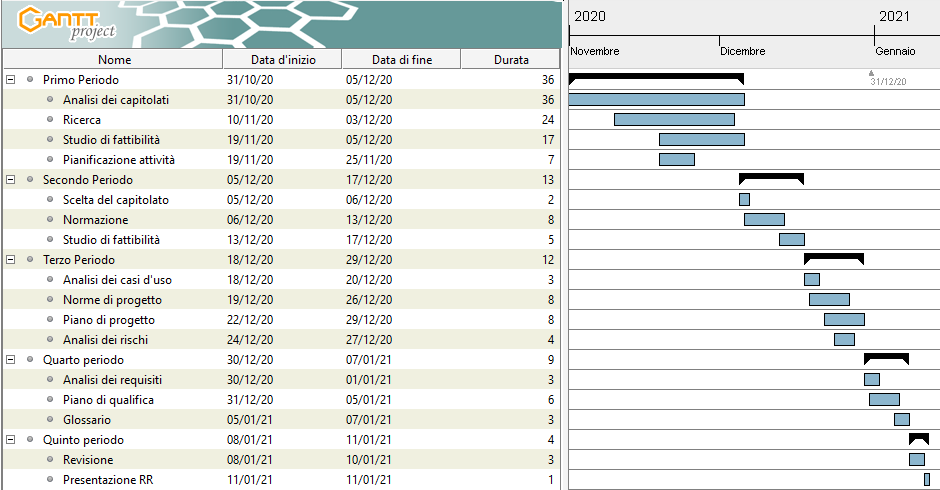
\includegraphics[width=1.7\textwidth]{images/1_Analisi_dei_requisiti.png}
%	\caption{Analisi dei requisiti}
%	\end{figure}
	
	\newpage
%	\KOMAoptions{paper=portrait,pagesize}
	
	\subsection{Consolidamento dei Requisiti}
	L’attività di consolidamento dei requisiti ha inizio il giorno 12-01-2021, successivamente alla consegna
	del materiale in ingresso alla revisione dei requisiti, ed è suddivisa in due periodi, con termine fissato
	per il giorno 17-01-2021, che precede la revisione dei requisiti del 18-01-2021.
	
	\subsection{Ruoli attivi}
	Durante questa attività è necessaria la presenza dei seguenti ruoli:
	\begin{itemize}
	\item responsabile;
	\item amministratore;
	\item analista.
	\end{itemize}

	\subsection{Periodi}
	L’attività di consolidamento dei requisiti è stata suddivisa nei seguenti due periodi:
	
	\subsubsection{Primo periodo dal 12-01-2021 al 15-01-2021}
	\begin{itemize}
	
	\item \textbf{Preparazione presentazione}: redazione della presentazione da portare in sede di revisione e
	studio individuale.
	
	\end{itemize}	
	
	\subsubsection{Secondo periodo dal 16-01-2021 al 17-01-2021}
	\begin{itemize}
		
	\item \textbf{Analisi dei requisiti}: revisione ed eventuale aggiornamento dei requisiti.
		
	\end{itemize}

	\newpage
	
%	\KOMAoptions{paper=landscape,pagesize}
%	\begin{figure}[h!]
%	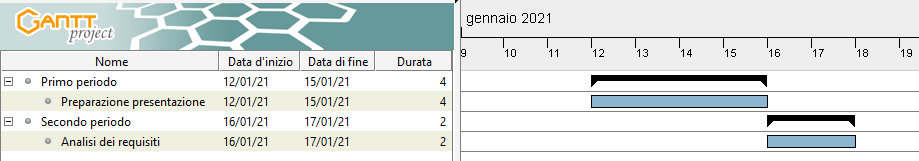
\includegraphics[width=1.7\textwidth]{images/2_Consolidamento_dei_requisiti.png}
%	\caption{Consolidamento dei requisiti}
%	\end{figure}

	\newpage
%	\KOMAoptions{paper=portrait,pagesize}

	
	\subsection{Progettazione della Technology Baseline}
	L’attività di progettazione della technology baseline ha inizio il giorno 19-01-2021, successivamente
	alla revisione dei requisiti, ed è suddivisa in tre periodi, con termine fissato per il giorno 07-01-2021,
	che precede la revisione di progettazione del 08-03-2021.
	
	\subsubsection{Ruoli attivi}
	Durante questa attività è necessaria la presenza dei seguenti ruoli:
	\begin{itemize}
	\item responsabile;
	\item amministratore;
	\item analista;
	\item progettista;
	\item programmatore;
	\item verificatore;
	\end{itemize}

	\subsubsection{Periodi}
	L’attività di progettazione della technology baseline è stata suddivisa nei seguenti periodi:
	
	\subsubsection{Primo periodo dal 19-01-2021 al 11-02-2021}
	\begin{itemize}
	\item \textbf{Normazione}: revisione ed eventuale aggiornamento delle norme;
	\item \textbf{Aggiornamento della pianificazione};
	\item \textbf{Aggiornamento della qualità};
	\item {Analisi dei requisiti}: revisione ed eventuale aggiornamento dei casi d’uso e dei requisiti, in base
	alle indicazioni ricevute;
	\item \textbf{Ricerca}: studio autonomo degli strumenti e le tecnologie da utilizzare per lo sviluppo del
	progetto;
	\item \textbf{Progettazione};
	\item \textbf{Verifica}: controllo della qualità di tutti i prodotti sviluppati durante il periodo attuale.
	\end{itemize}

	\subsubsection{Secondo periodo dal 12-02-2021 al 03-03-2021}
	\begin{itemize}
	\item \textbf{Normazione}: aggiornamento delle norme;
	\item \textbf{Progettazione}: progettazione del PROOF OF CONCEPTG che deve essere implementato;
	\item \textbf{Aggiornamento della pianificazione};
	\item \textbf{Codifica}: implementazione del PROOF OF CONCEPTG progettato;
	\item \textbf{Stesura della lettera di presentazione}: scrittura della lettera di presentazione con la quale ci
	si candida alla revisione di progettazione;
	\item \textbf{Verifica}: controllo della qualità di tutti i prodotti sviluppati durante il periodo attuale.
	\end{itemize}	
	
	\subsubsection{Terzo periodo dal 04-03-2021 al 07-03-2021}
	\begin{itemize}
	\item \textbf{Preparazione presentazione}: redazione della presentazione da portare in sede di revisione e
	studio individuale.
	\end{itemize}

	\begin{landscape}
	\newpage
	
	\begin{figure}[h!]
	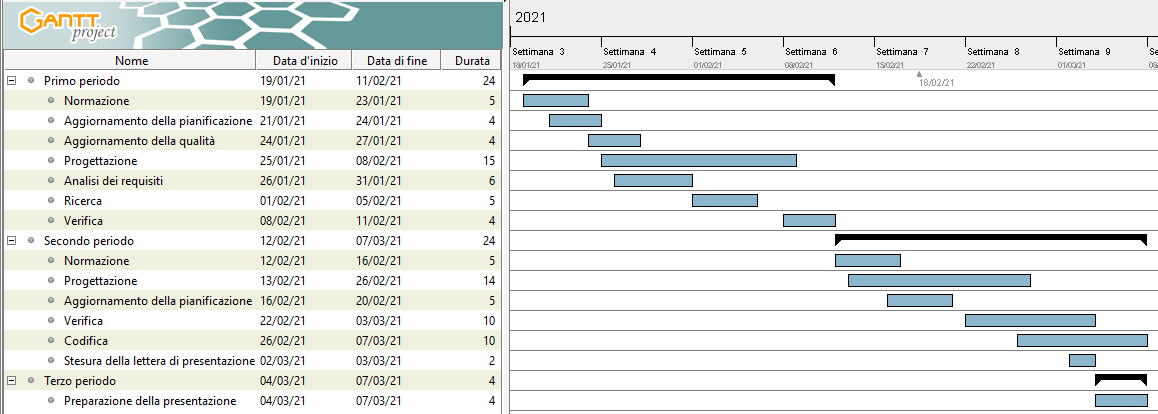
\includegraphics[width=1.7\textwidth]{images/3_Progettazione_della_Technology.png}
	\caption{Progettazione della Technology}
	\end{figure}
	\end{landscape}
	
	\newpage	
	
	\subsection{Progettazione di dettaglio e Codifica}
	L’attività di progettazione di dettaglio e codifica ha inizio il giorno 09-03-2021, successivamente alla
	revisione di progettazione, ed è suddivisa in tre periodi, con termine fissato per il giorno 08-04-2021,
	che precede la revisione di qualifica del 09-04-2021.
	
	\subsubsection{Ruoli attivi}
	Durante questa attività è necessaria la presenza dei seguenti ruoli:
	\begin{itemize}
	\item responsabile;
	\item amministratore;
	\item progettista;
	\item programmatore;
	\item verificatore;
	\end{itemize}

	\subsubsection{Periodi}
	L’attività di progettazione di dettaglio e codifica è stata suddivisa nei seguenti periodi:
	\subsubsection{Primo periodo dal 09-03-2021 al 18-03-2021}
	\begin{itemize}
		\item \textbf{Normazione}: aggiornamento delle norme;
		\item \textbf{Aggiornamento della pianificazione};
		\item \textbf{Aggiornamento della qualità};
		\item \textbf{Progettazione}: miglioramento incrementale della progettazione fatta per il PROOF OF CONCEPTG;
		\item \textbf{Codifica}: implementazione prodotto software e test;
		\item \textbf{Scrittura manuale}: prima stesura;
		\item \textbf{Verifica}: controllo della qualità di tutti i prodotti sviluppati durante il periodo attuale.
	\end{itemize}

	\subsubsection{Secondo periodo dal 19-03-2021 al 30-03-2021}
	\begin{itemize}
	\item \textbf{Normazione}: aggiornamento delle norme;
	\item \textbf{Aggiornamento della pianificazione};
	\item \textbf{Progettazione}: miglioramento incrementale della progettazione tramite DESIGN PATTERNG;
	\item \textbf{Codifica}: primo rilascio;
	\item \textbf{Aggiornamento manuale};
	\item \textbf{Stesura della lettera di presentazione}: scrittura della lettera di presentazione con la quale ci
	si candida alla revisione di qualifica;
	\item \textbf{Verifica}: controllo della qualità di tutti i prodotti sviluppati durante il periodo attuale.
	\end{itemize}

	\subsubsection{Terzo periodo dal 31-03-2021 al 08-04-2021}
	\begin{itemize}
	\item \textbf{Preparazione presentazione}: redazione della presentazione da portare in sede di revisione e
	studio individuale.
	\end{itemize}

	\newpage
%	\KOMAoptions{paper=landscape,pagesize}
%	\begin{figure}[h!]
%	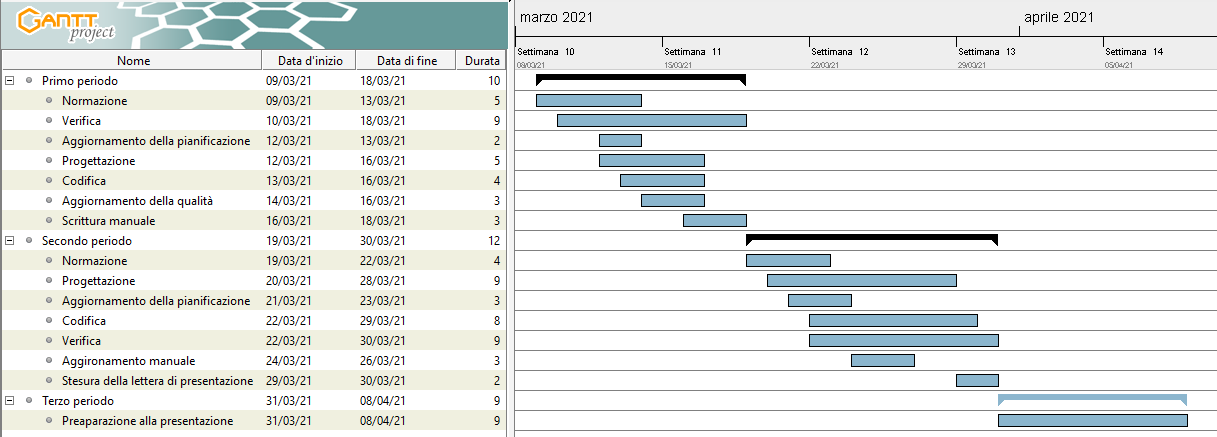
\includegraphics[width=1.7\textwidth]{images/4_Progettazione_e_codifica.png}
%	\caption{Progettazione e codifica}
%	\end{figure}
	
	\newpage
%	\KOMAoptions{paper=portrait,pagesize}
	
	\newpage

	\subsection{Validazione e Collaudo}
	L’attività di validazione e collaudo ha inizio il giorno 10-04-2021, successivamente alla revisione di
	qualifica, ed è suddivisa in tre periodi, con termine fissato per il giorno 09-05-2021, che precede la
	revisione di accettazione del 10-05-2021.
	
	\subsubsection{Ruoli attivi}
	Durante questa attività è necessaria la presenza dei seguenti ruoli:
	\begin{itemize}
		\item responsabile;
		\item amministratore;
		\item progettista;
		\item programmatore;
		\item verificatore;
	\end{itemize}

	\subsubsection{Periodi}
	L’attività di validazione e collaudo è stata suddivisa nei seguenti periodi:
	\subsubsection{Primo periodo dal 10-04-2021 al 23-04-2021}
	\begin{itemize}
		\item \textbf{Normazione}: revisione ed eventuale aggiornamento delle norme;
		\item \textbf{Aggiornamento} della pianificazione;
		\item \textbf{Aggiornamento della qualità};
		\item \textbf{Completamento progettazione};
		\item \textbf{Verifica}: controllo della qualità di tutti i prodotti sviluppati durante il periodo attuale.
	\end{itemize}

	\subsubsection{Secondo periodo dal 24-04-2021 al 02-05-2021}
	\begin{itemize}
		\item \textbf{Codifica}: rilascio ultima versione;
		\item \textbf{Completamento manuale};
		\item \textbf{Verifica}: controllo della qualità di tutti i prodotti sviluppati durante il periodo attuale, in
		particolare sono eseguiti i test per la verifica del software.
	\end{itemize}

	\subsubsection{Terzo periodo dal 03-05-2021 al 09-05-2021}
	\begin{itemize}
		\item \textbf{Preparazione presentazione}: redazione della presentazione da portare in sede di revisione e
		studio individuale.
	\end{itemize}

	\newpage
%	\KOMAoptions{paper=landscape,pagesize}
%	\begin{figure}[h!]
%	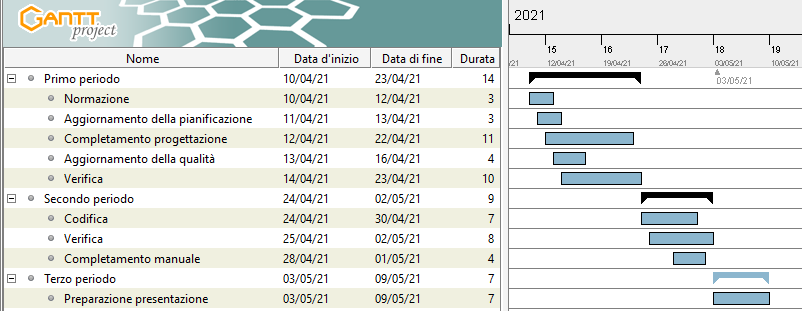
\includegraphics[width=1.7\textwidth]{images/5_Validazione_e_collaudo.png}
%	\caption{Validazione e collaudo}
%	\end{figure}
	
	\newpage
%	\KOMAoptions{paper=portrait,pagesize}
	\newpage

	\section{Preventivo}
	
Nelle varie sezioni di questo capitolo è riportato il preventivo per ogni fase di lavoro del progetto con un riepilogo finale.\\
\\Le 5 fasi previste sono:
\begin{enumerate}
	\item Analisi dei requisiti;
	\item Analisi di dettaglio;
	\item Codifica \glock{Technlogy Baseline};
	\item Incrementi, suddivisi in:
	\begin{itemize}
		\item Incremento I - Incremento II;
		\item Incremento III;
		\item Incremento IV - Incremento V;
		\item Incremento VI - Incremento VII;
		\item Incremento VIII - Incremento IX;
		
	\end{itemize}
	\item Validazione.
\end{enumerate}
Ognuna di esse è specificata come segue:
\begin{itemize}
	\item tabella riepilogativa delle ore per ruolo/persona;
	\item grafico a barre delle ore svolte dai membri del gruppo nei vari ruoli;
	\item tabella del prospetto economico suddiviso per ruoli;
	\item grafico a torta del costo suddiviso per ruoli.
\end{itemize}
In molte delle tabelle e figure proposte, i ruoli sono stati abbreviati in questo modo:
\begin{itemize}
	\item \textbf{Re}: Responsabile;
	\item \textbf{Am}: Amministratore;
	\item \textbf{An}: Analista;
	\item \textbf{Pg}: Progettista;
	\item \textbf{Pr}: Programmatore;
	\item \textbf{Ve}: Verificatore.
\end{itemize}

\newpage

\subsection{Analisi dei requisiti}
	
	\subsubsection{Prospetto orario}
			
		\begin{table} [h!]
			\rowcolors{2}{gray!25}{gray!6}
			\begin{center}
				\begin{tabular} { m{3.5cm} c c c c c c c }
					\rowcolor{lightgray}
					\textbf{Nome} & \textbf{Re} & \textbf{Am} & \textbf{An} & \textbf{Pg} & \textbf{Pr} & \textbf{Ve} & \textbf{Totale} \\
					Matteo Alba &0 & 8 & 8 &0 & 0& 10 & 26\\
					Giacomo Bulbarelli & 7 & 6 & 8 & 0& 0& 5 & 26 \\
					Alessandro Chimetto & 7 &0 & 11 &0 & 0& 8 & 26 \\
					Alessandro Dindinelli &0 & 4 & 12 &0 & 0& 10 & 26 \\
					Lucia Fenu &0 & 6 & 10 &0 & 0& 10 & 26 \\
					Paolo Scanferlato & 5 & 7 & 6 & 0& 0& 8 & 26 \\
					Valton Tahiraj & 6 & 5 & 7 &0 & 0& 8 & 26 \\
					\textbf{Ore totali Ruolo} & \textbf{25} & \textbf{36} & \textbf{62} & \textbf{0} & \textbf{0}& \textbf{59} & \textbf{182}
				\end{tabular}
				\caption{Preventivo - Analisi dei requisiti - ore per persona/ruolo}
			\end{center}
		\end{table}

		\begin{figure} [h!]
			\centering
			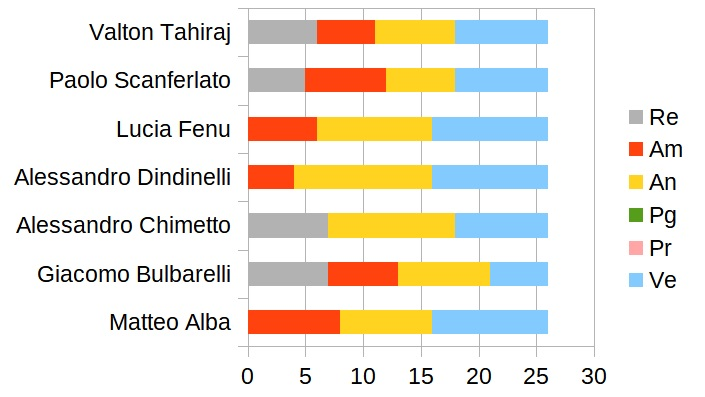
\includegraphics[width=0.8\textwidth]{res/img/grafici/analisi_dei_requisiti_ore_ruolo.jpg}
			\caption{Preventivo - Analisi dei requisiti - ore per persona/ruolo} 
		\end{figure}

	\newpage

	\subsubsection{Prospetto economico}

		\begin{table} [h!] % QUESTA RICHIEDE \usepackage{eurosym} IN config.tex
			\rowcolors{2}{gray!25}{gray!6}
			\begin{center}
				\begin{tabular} { m{3cm} >{\centering}m{1.5cm} c }
					\rowcolor{lightgray}
					\textbf{Ruolo} & \textbf{Ore} & \textbf{Costo in \euro} \\
					Responsabile & 25 & 750,00 \\
					Amministratore & 36 & 720,00 \\
					Analista & 62 & 1550,00 \\
					Progettista & 0&0 \\
					Programmatore &0 & 0\\
					Verificatore & 59 & 885,00 \\
					\textbf{Totale} & \textbf{182} & \textbf{3905,00} \\
				\end{tabular}
				\caption{Preventivo - Analisi dei requisiti - costo per ruolo}
			\end{center}
		\end{table}
	
		\begin{figure} [h!]
			\centering
			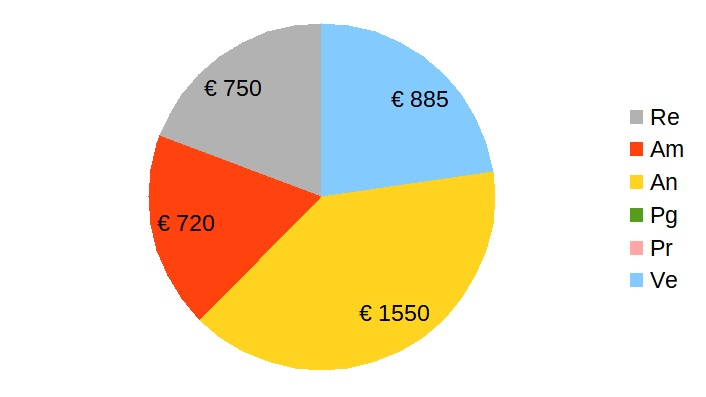
\includegraphics[width=0.8\textwidth]{res/img/grafici/analisi_dei_requisiti_costi.jpg}
			\caption{Preventivo - Analisi dei requisiti - costo per ruolo} 
		\end{figure}

\newpage

\subsection{Analisi di dettaglio}

	\subsubsection{Prospetto orario}
	
		\begin{table} [h!]
			\rowcolors{2}{gray!25}{gray!6}
			\begin{center}
				\begin{tabular} { m{3.5cm} c c c c c c c }
					\rowcolor{lightgray}
					\textbf{Nome} & \textbf{Re} & \textbf{Am} & \textbf{An} & \textbf{Pg} & \textbf{Pr} & \textbf{Ve} & \textbf{Totale} \\
					Matteo Alba & 2 & 0&0 & 0&0 & 4 & \textbf{6} \\
					Giacomo Bulbarelli & 0& 2 & 4 &0 & 0&0 & \textbf{6} \\
					Alessandro Chimetto &0& 5 & 1 &0 &0 &0 & \textbf{6} \\
					Alessandro Dindinelli & 3 &0 & 1 &0 &0 & 2 & \textbf{6} \\
					Lucia Fenu & 1 &0 & 3 &0 & 0& 2 & \textbf{6} \\
					Paolo Scanferlato &0 & 0& 2 & 0&0 & 4 & \textbf{6} \\
					Valton Tahiraj & 0& 0& 3 &0 & 0& 3 & \textbf{6} \\
					\textbf{Ore totali Ruolo} & \textbf{6} & \textbf{7} & \textbf{14} & \textbf{0} & \textbf{0}& \textbf{15} & \textbf{42}
				\end{tabular}
				\caption{Preventivo - Analisi di dettaglio - ore per persona/ruolo}
			\end{center}
		\end{table}
	
		\begin{figure} [h!]
			\centering
			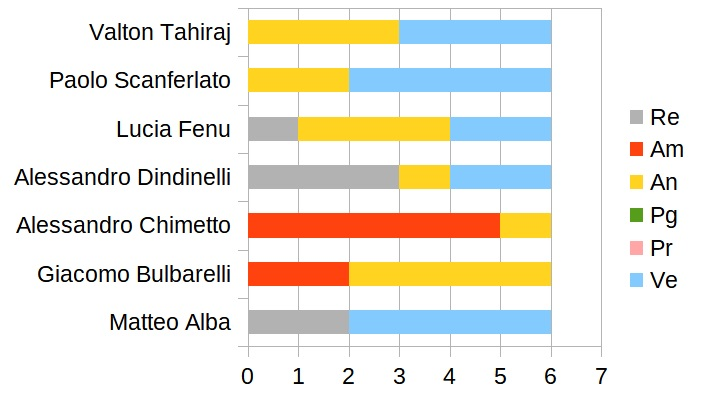
\includegraphics[width=0.8\textwidth]{res/img/grafici/consolidamento_dei_requisiti_ore_ruolo.jpg}
			\caption{Preventivo - Analisi di dettaglio -ore per persona/ruolo} 
		\end{figure}
		
	\newpage

	\subsubsection{Prospetto economico}
	
		\begin{table} [h!] % QUESTA RICHIEDE \usepackage{eurosym} IN config.tex
			\rowcolors{2}{gray!25}{gray!6}
			\begin{center}
				\begin{tabular} { m{3cm} >{\centering}m{1.5cm} c }
					\rowcolor{lightgray}
					\textbf{Ruolo} & \textbf{Ore} & \textbf{Costo in \euro} \\
					Responsabile & 6 & 180,00 \\
					Amministratore & 7 & 140,00 \\
					Analista & 14 & 350,00 \\
					Progettista &0 & 0\\
					Programmatore &0 & 0\\
					Verificatore & 15 & 225,00 \\
					\textbf{Totale} & \textbf{42} & \textbf{895,00} \\
				\end{tabular}
				\caption{Preventivo - Analisi di dettaglio - costo per ruolo}
			\end{center}
		\end{table}
	
		\begin{figure} [h!]
			\centering
			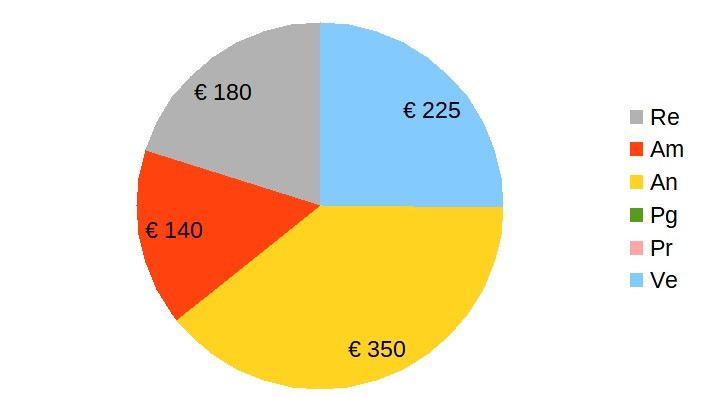
\includegraphics[width=0.8\textwidth]{res/img/grafici/consolidamento_dei_requisiti_costi.jpg}
			\caption{Preventivo - Analisi di dettaglio - costo per ruolo} 
		\end{figure}

\newpage

\subsection{Codifica \glock{Technlogy Baseline}}

	\subsubsection{Prospetto orario}

		\begin{table} [h!]
			\rowcolors{2}{gray!25}{gray!6}
			\begin{center}
				\begin{tabular} { m{3.5cm} c c c c c c c }
					\rowcolor{lightgray}
					\textbf{Nome} & \textbf{Re} & \textbf{Am} & \textbf{An} & \textbf{Pg} & \textbf{Pr} & \textbf{Ve} & \textbf{Totale} \\
					Matteo Alba & 8 &0 & 5 & 3 & 5 & 6 & \textbf{27} \\
					Giacomo Bulbarelli & 3 & 0& 5 & 7 & 5 & 7 & \textbf{27} \\
					Alessandro Chimetto & 0& 2 & 4 & 6 & 6 & 9 & \textbf{27} \\
					Alessandro Dindinelli & 2 & 4 & 0& 7 & 7 & 7 & \textbf{27} \\
					Lucia Fenu &0 & 2 & 2 & 7 & 7 & 9 & \textbf{27} \\
					Paolo Scanferlato & 2 & 3 & 3 & 6 & 4 & 9 & \textbf{27} \\
					Valton Tahiraj &0 & 3 & 4 & 3 & 6 & 11 & \textbf{27} \\
					\textbf{Ore totali Ruolo} & \textbf{15} & \textbf{14} & \textbf{23} & \textbf{39} & \textbf{40}& \textbf{58} & \textbf{189}
				\end{tabular}
				\caption{Preventivo - Codifica \glock{Technlogy Baseline} - ore per persona/ruolo}
			\end{center}
		\end{table}
		
		\begin{figure} [h!]
			\centering
			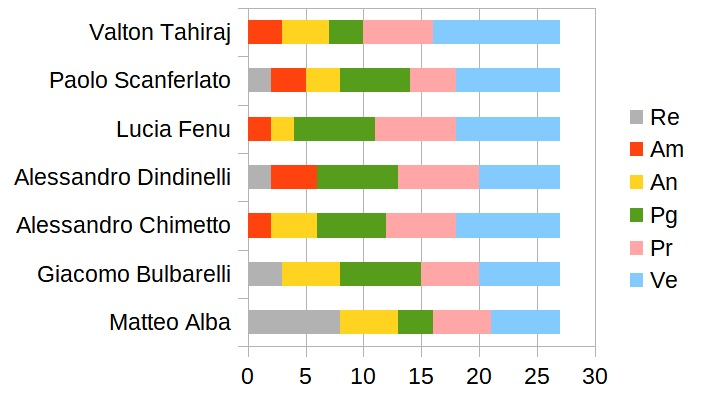
\includegraphics[width=0.8\textwidth]{res/img/grafici/progettazione_architetturale_ore_ruolo.jpg}
			\caption{Preventivo - Codifica \glock{Technlogy Baseline} - ore per persona/ruolo} 
		\end{figure}
		
	\newpage
	
	\subsubsection{Prospetto economico}
	
		\begin{table} [h!] % QUESTA RICHIEDE \usepackage{eurosym} IN config.tex
			\rowcolors{2}{gray!25}{gray!6}
			\begin{center}
				\begin{tabular} { m{3cm} >{\centering}m{1.5cm} c }
					\rowcolor{lightgray}
					\textbf{Ruolo} & \textbf{Ore} & \textbf{Costo in \euro} \\
					Responsabile & 15 & 450,00 \\
					Amministratore & 14 & 280,00 \\
					Analista & 23 & 575,00 \\
					Progettista & 39 & 858,00 \\
					Programmatore & 40 & 600,00 \\
					Verificatore & 58 & 870,00 \\
					\textbf{Totale} & \textbf{189} & \textbf{3633,00} \\
				\end{tabular}
				\caption{Preventivo - Codifica \glock{Technlogy Baseline} - costo per ruolo}
			\end{center}
		\end{table}
	
		\begin{figure} [h!]
			\centering
			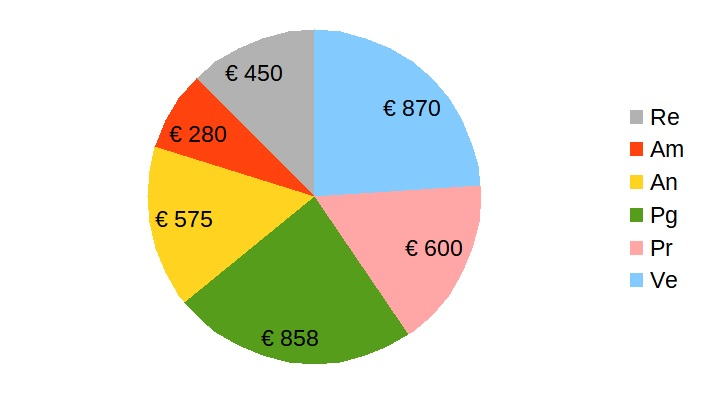
\includegraphics[width=0.8\textwidth]{res/img/grafici/progettazione_architetturale_costi.jpg}
			\caption{Preventivo - Codifica \glock{Technlogy Baseline} - costo per ruolo} 
		\end{figure}
	
\newpage



\subsection{Incremento I - Incremento II}
\subsubsection{Prospetto orario}

	\begin{table} [h!]
	\rowcolors{2}{gray!25}{gray!6}
	\begin{center}
		\begin{tabular} { m{3.5cm} c c c c c c c }
			\rowcolor{lightgray}
			\textbf{Nome} & \textbf{Re} & \textbf{Am} & \textbf{An} & \textbf{Pg} & \textbf{Pr} & \textbf{Ve} & \textbf{Totale} \\
			Matteo Alba & 0&2 & 0& 0&4 & 4 & 10 \\
			Giacomo Bulbarelli & 0& 0& 0& 4 & 3 & 3 & 10 \\
			Alessandro Chimetto & 0& 0& 0& 5 & 3 & 3 & 10 \\
			Alessandro Dindinelli & 0& 0& 0& 3 & 5 &2 & 10 \\
			Lucia Fenu & 0& 0& 0& 4 & 3 & 3 & 10 \\
			Paolo Scanferlato &2 & 0& 0& 3 & 3 & 2 & 10 \\
			Valton Tahiraj & 2& 0&2 & 0& 4 & 2 & 10 \\
			\textbf{Ore totali Ruolo} & \textbf{4} & \textbf{2} & \textbf{2} & \textbf{19} & \textbf{25}& \textbf{18} & \textbf{70}
		\end{tabular}
		\caption{Preventivo - Incremento I - Incremento II - ore per persona/ruolo}
	\end{center}
\end{table}
	\begin{figure} [h!]
	\centering
	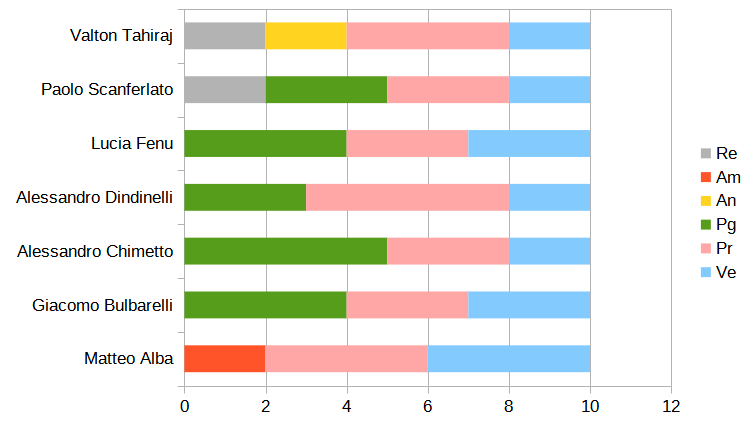
\includegraphics[width=0.8\textwidth]{res/img/preventivi/1e2-barre.png}
	\caption{Preventivo - Incremento I - Incremento II - ore per persona/ruolo} 
\end{figure}

\newpage

\subsubsection{Prospetto economico}
	\begin{table} [h!] % QUESTA RICHIEDE \usepackage{eurosym} IN config.tex
	\rowcolors{2}{gray!25}{gray!6}
	\begin{center}
		\begin{tabular} { m{3cm} >{\centering}m{1.5cm} c }
			\rowcolor{lightgray}
			\textbf{Ruolo} & \textbf{Ore} & \textbf{Costo in \euro} \\
			Responsabile &4 & 120,00 \\
			Amministratore & 2 & 40,00 \\
			Analista &2 &50,00 \\
			Progettista & 19 & 418,00 \\
			Programmatore & 25 & 375,00 \\
			Verificatore & 18 & 270,00 \\
			\textbf{Totale} & \textbf{70} & \textbf{1273,00} \\
		\end{tabular}
		\caption{Preventivo - Incremento I - Incremento II - costo per ruolo}
	\end{center}
\end{table}

\begin{figure} [h!]
	\centering
	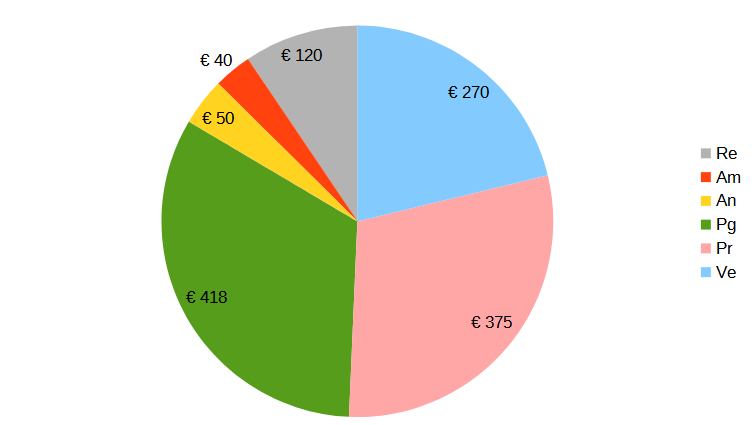
\includegraphics[width=0.8\textwidth]{res/img/preventivi/1e2-torta.png}
	\caption{Preventivo - Incremento I - Incremento II - costo per ruolo} 
\end{figure}


\newpage
\subsection{Incremento III}
\subsubsection{Prospetto orario}

	\begin{table} [h!]
	\rowcolors{2}{gray!25}{gray!6}
	\begin{center}
		\begin{tabular} { m{3.5cm} c c c c c c c }
			\rowcolor{lightgray}
			\textbf{Nome} & \textbf{Re} & \textbf{Am} & \textbf{An} & \textbf{Pg} & \textbf{Pr} & \textbf{Ve} & \textbf{Totale} \\
			Matteo Alba & 0& 0& 0& 4& 0& 5& 9 \\
			Giacomo Bulbarelli & 0& 3& 0& 2& 4& 0& 9 \\
			Alessandro Chimetto & 0& 0& 2& 0& 4& 3& 9 \\
			Alessandro Dindinelli & 3& 0& 0& 0& 4&2 & 9 \\
			Lucia Fenu & 0& 0& 0& 4 & 5 & 0 & 9 \\
			Paolo Scanferlato &0 & 0& 0& 4 & 5 & 0 & 9 \\
			Valton Tahiraj & 0& 0&0 &4 & 0 & 5 & 9 \\
			\textbf{Ore totali Ruolo} & \textbf{3} & \textbf{3} & \textbf{2} & \textbf{18} & \textbf{22}& \textbf{15} & \textbf{63}
		\end{tabular}
		\caption{Preventivo - Incremento III - ore per persona/ruolo}
	\end{center}
\end{table}
\begin{figure} [h!]
	\centering
	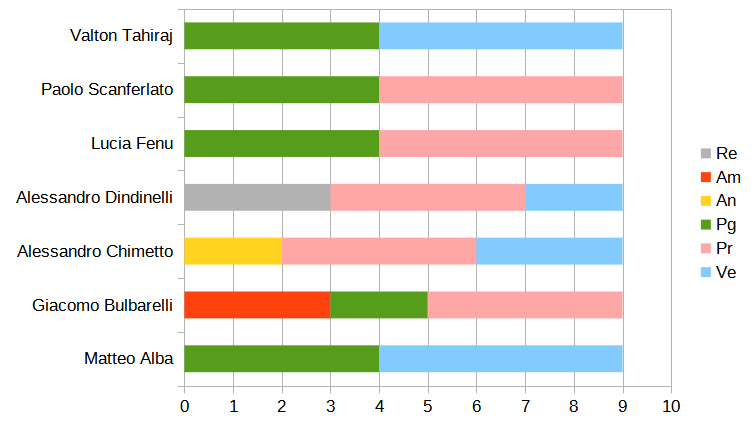
\includegraphics[width=0.8\textwidth]{res/img/preventivi/3-barre.png}
	\caption{Preventivo - Incremento III - ore per persona/ruolo} 
\end{figure}

\newpage

\subsubsection{Prospetto economico}
	\begin{table} [h!] % QUESTA RICHIEDE \usepackage{eurosym} IN config.tex
	\rowcolors{2}{gray!25}{gray!6}
	\begin{center}
		\begin{tabular} { m{3cm} >{\centering}m{1.5cm} c }
			\rowcolor{lightgray}
			\textbf{Ruolo} & \textbf{Ore} & \textbf{Costo in \euro} \\
			Responsabile &3 & 90,00 \\
			Amministratore & 3 & 60,00 \\
			Analista &2 &50,00 \\
			Progettista & 18 & 396,00 \\
			Programmatore & 22 & 330,00 \\
			Verificatore & 15 & 225,00 \\
			\textbf{Totale} & \textbf{63} & \textbf{1151,00} \\
		\end{tabular}
		\caption{Preventivo - Incremento I - Incremento II - costo per ruolo}
	\end{center}
\end{table}

\begin{figure} [h!]
	\centering
	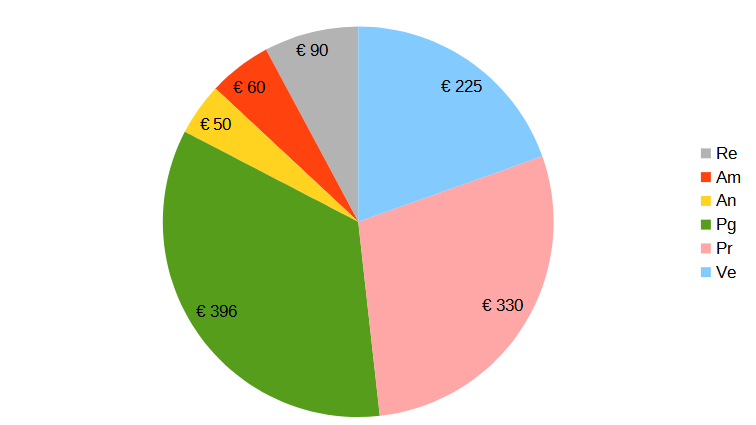
\includegraphics[width=0.8\textwidth]{res/img/preventivi/3-torta.png}
	\caption{Preventivo - Incremento III - costo per ruolo} 
\end{figure}
\newpage
\subsection{Incremento IV - Incremento V}
\subsubsection{Prospetto orario}

\begin{table} [h!]
	\rowcolors{2}{gray!25}{gray!6}
	\begin{center}
		\begin{tabular} { m{3.5cm} c c c c c c c }
			\rowcolor{lightgray}
			\textbf{Nome} & \textbf{Re} & \textbf{Am} & \textbf{An} & \textbf{Pg} & \textbf{Pr} & \textbf{Ve} & \textbf{Totale} \\
			Matteo Alba &2 &0 & 0& 5 &5 & 0 & 12 \\
			Giacomo Bulbarelli & 0 &0 & 0& 2 & 5 & 5 & 12 \\
			Alessandro Chimetto & 0 & 2& 0& 5 & 5 & 0& 12 \\
			Alessandro Dindinelli & 0& 0 & 2& 4 & 3 &3 & 12 \\
			Lucia Fenu & 2 & 0 &0 & 3 & 3 & 4 & 12 \\
			Paolo Scanferlato &0 & 0 &0 & 3 & 4 & 5 & 12\\
			Valton Tahiraj & 0& 0 &0 & 4 & 5 & 3 & 12 \\
			\textbf{Ore totali Ruolo} & \textbf{4} & \textbf{2} & \textbf{2} & \textbf{26} & \textbf{30}& \textbf{20} & \textbf{84}
		\end{tabular}
		\caption{Preventivo - Incremento IV - Incremento V - ore per persona/ruolo}
	\end{center}
\end{table}
\begin{figure} [h!]
	\centering
	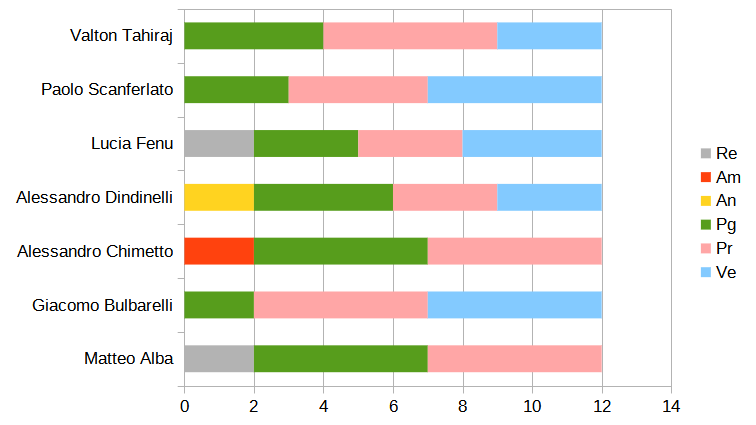
\includegraphics[width=0.8\textwidth]{res/img/preventivi/4e5-barre.png}
	\caption{Preventivo - Incremento IV - Incremento V - ore per persona/ruolo} 
\end{figure}

\newpage

\subsubsection{Prospetto economico}
	\begin{table} [h!] % QUESTA RICHIEDE \usepackage{eurosym} IN config.tex
	\rowcolors{2}{gray!25}{gray!6}
	\begin{center}
		\begin{tabular} { m{3cm} >{\centering}m{1.5cm} c }
			\rowcolor{lightgray}
			\textbf{Ruolo} & \textbf{Ore} & \textbf{Costo in \euro} \\
			Responsabile &4 & 120,00 \\
			Amministratore & 2 & 40,00 \\
			Analista &2 &50,00 \\
			Progettista & 26 & 572,00 \\
			Programmatore & 30 & 450,00 \\
			Verificatore & 20 & 300,00 \\
			\textbf{Totale} & \textbf{63} & \textbf{1532,00} \\
		\end{tabular}
		\caption{Preventivo - Incremento IV - Incremento V - costo per ruolo}
	\end{center}
\end{table}

\begin{figure} [h!]
	\centering
	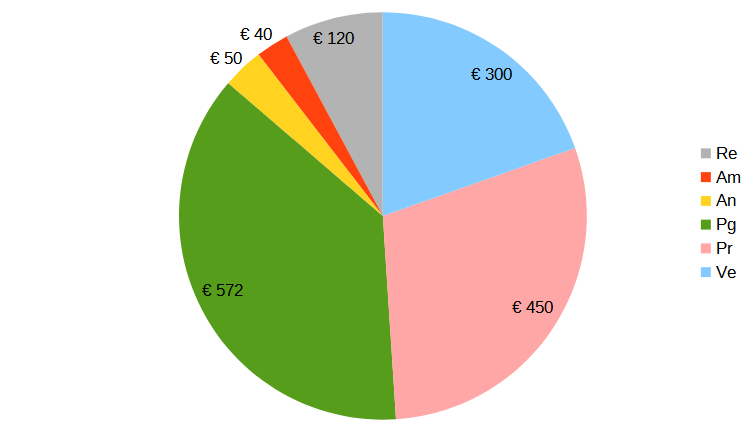
\includegraphics[width=0.8\textwidth]{res/img/preventivi/4e5-torta.png}
	\caption{Preventivo - Incremento IV - Incremento V - costo per ruolo} 
\end{figure}
\newpage
\subsection{Incremento VI - Incremento VII}
\subsubsection{Prospetto orario}

\begin{table} [h!]
	\rowcolors{2}{gray!25}{gray!6}
	\begin{center}
		\begin{tabular} { m{3.5cm} c c c c c c c }
			\rowcolor{lightgray}
			\textbf{Nome} & \textbf{Re} & \textbf{Am} & \textbf{An} & \textbf{Pg} & \textbf{Pr} & \textbf{Ve} & \textbf{Totale} \\
			Matteo Alba &0 &0 & 2& 0 &5 & 3 & 10 \\
			Giacomo Bulbarelli & 2&0 & 0& 3 & 5 & 0 & 10 \\
			Alessandro Chimetto & 2 & 0& 0& 3 & 0 & 5& 10 \\
			Alessandro Dindinelli & 0& 0 & 0& 4 & 3 &3 & 10 \\
			Lucia Fenu & 0 & 0 &0 & 5 & 5 & 0 & 10 \\
			Paolo Scanferlato &0 & 0 &0 & 4 & 3 & 3 & 10\\
			Valton Tahiraj & 0& 2 &0 & 0 & 4 & 4 & 10 \\
			\textbf{Ore totali Ruolo} & \textbf{4} & \textbf{2} & \textbf{2} & \textbf{19} & \textbf{25}& \textbf{18} & \textbf{70}
		\end{tabular}
		\caption{Preventivo - Incremento VI - Incremento VII - ore per persona/ruolo}
	\end{center}
\end{table}
\begin{figure} [h!]
	\centering
	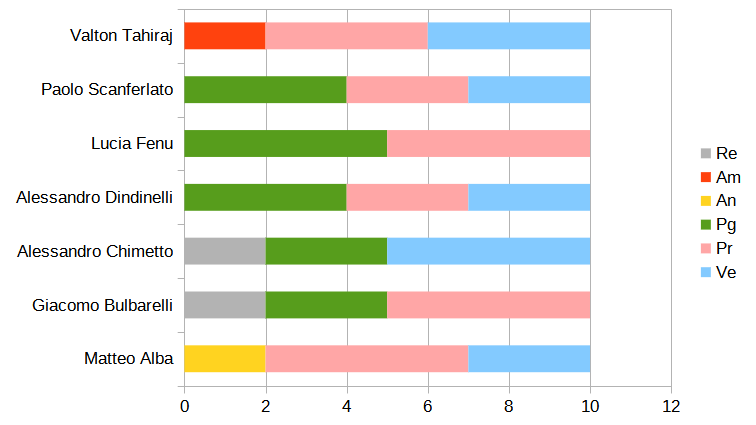
\includegraphics[width=0.8\textwidth]{res/img/preventivi/6e7-barre.png}
	\caption{Preventivo - Incremento VI - Incremento VII - ore per persona/ruolo} 
\end{figure}

\newpage
\subsubsection{Prospetto economico}

	\begin{table} [h!] % QUESTA RICHIEDE \usepackage{eurosym} IN config.tex
	\rowcolors{2}{gray!25}{gray!6}
	\begin{center}
		\begin{tabular} { m{3cm} >{\centering}m{1.5cm} c }
			\rowcolor{lightgray}
			\textbf{Ruolo} & \textbf{Ore} & \textbf{Costo in \euro} \\
			Responsabile &4 & 120,00 \\
			Amministratore & 2 & 40,00 \\
			Analista &2 &50,00 \\
			Progettista & 19 & 418,00 \\
			Programmatore & 25 & 375,00 \\
			Verificatore &18 & 270,00 \\
			\textbf{Totale} & \textbf{70} & \textbf{1273,00} \\
		\end{tabular}
		\caption{Preventivo - Incremento VI - Incremento VII - costo per ruolo}
	\end{center}
\end{table}

\begin{figure} [h!]
	\centering
	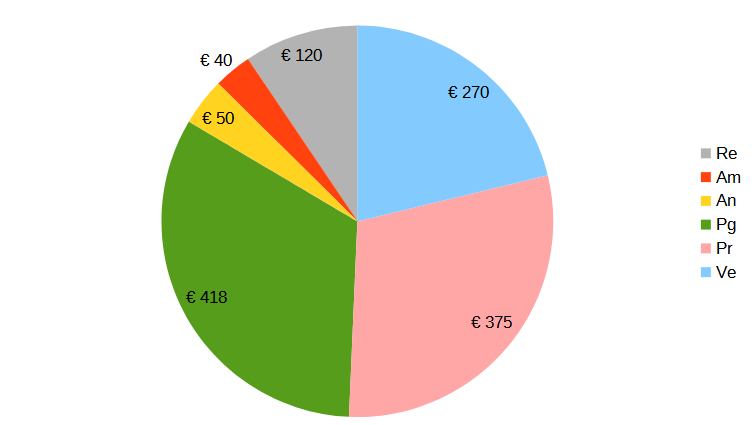
\includegraphics[width=0.8\textwidth]{res/img/preventivi/6e7-torta.png}
	\caption{Preventivo - Incremento VI - Incremento VII - costo per ruolo} 
\end{figure}
\newpage
\subsection{Incremento VIII - Incremento IX}
\subsubsection{Prospetto orario}

\begin{table} [h!]
	\rowcolors{2}{gray!25}{gray!6}
	\begin{center}
		\begin{tabular} { m{3.5cm} c c c c c c c }
			\rowcolor{lightgray}
			\textbf{Nome} & \textbf{Re} & \textbf{Am} & \textbf{An} & \textbf{Pg} & \textbf{Pr} & \textbf{Ve} & \textbf{Totale} \\
			Matteo Alba &0 &3 & 0& 3 &2 & 4 & 12 \\
			Giacomo Bulbarelli & 0&3 & 0& 3 & 2 & 4 & 12 \\
			Alessandro Chimetto & 2 & 2& 3& 0 & 0 & 5& 12 \\
			Alessandro Dindinelli & 0& 4 & 0& 3 & 2 &3 & 12 \\
			Lucia Fenu & 0& 4 & 0& 3 & 2 &3 & 12 \\
			Paolo Scanferlato &3 & 4 &0 & 0 & 0 & 5 & 12\\
			Valton Tahiraj & 3& 0 &2 & 2 & 0 & 5 & 12 \\
			\textbf{Ore totali Ruolo} & \textbf{8} & \textbf{20} & \textbf{5} & \textbf{14} & \textbf{8}& \textbf{29} & \textbf{84}
		\end{tabular}
		\caption{Preventivo - Incremento VIII - Incremento IX - ore per persona/ruolo}
	\end{center}
\end{table}
\begin{figure} [h!]
	\centering
	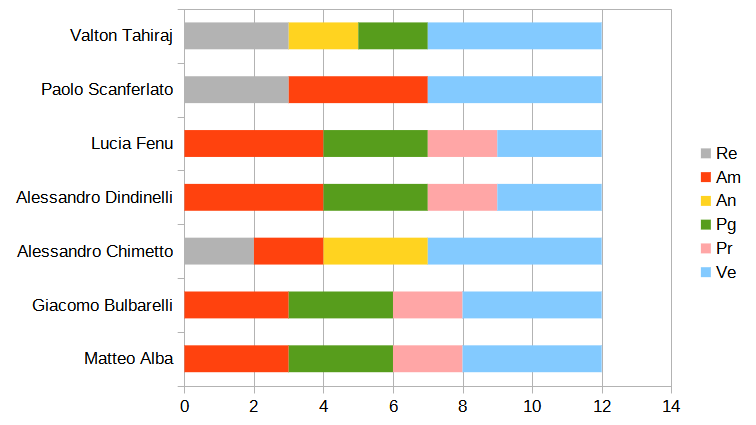
\includegraphics[width=0.8\textwidth]{res/img/preventivi/8e9-barre.png}
	\caption{Preventivo - Incremento VIII - Incremento IX - ore per persona/ruolo} 
\end{figure}

\newpage
\subsubsection{Prospetto economico}
	\begin{table} [h!] % QUESTA RICHIEDE \usepackage{eurosym} IN config.tex
	\rowcolors{2}{gray!25}{gray!6}
	\begin{center}
		\begin{tabular} { m{3cm} >{\centering}m{1.5cm} c }
			\rowcolor{lightgray}
			\textbf{Ruolo} & \textbf{Ore} & \textbf{Costo in \euro} \\
			Responsabile &8 & 240,00 \\
			Amministratore & 20 & 400,00 \\
			Analista &5 &125,00 \\
			Progettista & 14 & 308,00 \\
			Programmatore & 8 & 120,00 \\
			Verificatore &29 & 435,00 \\
			\textbf{Totale} & \textbf{84} & \textbf{1628,00} \\
		\end{tabular}
		\caption{Preventivo - Incremento VIII - Incremento IX  - costo per ruolo}
	\end{center}
\end{table}

\begin{figure} [h!]
	\centering
	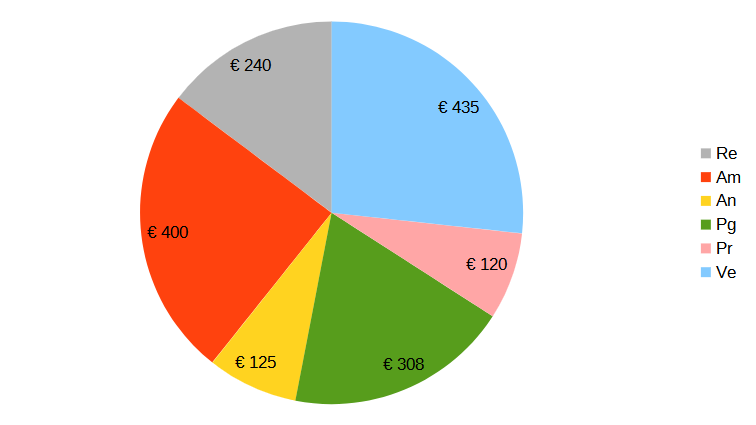
\includegraphics[width=0.8\textwidth]{res/img/preventivi/8e9-torta.png}
	\caption{Preventivo - Incremento VIII - Incremento IX  - costo per ruolo} 
\end{figure}
\newpage
\subsection{Validazione e collaudo}

	\subsubsection{Prospetto orario}

		\begin{table} [h!]
			\rowcolors{2}{gray!25}{gray!6}
			\begin{center}
				\begin{tabular} { m{3.5cm} c c c c c c c }
					\rowcolor{lightgray}
					\textbf{Nome} & \textbf{Re} & \textbf{Am} & \textbf{An} & \textbf{Pg} & \textbf{Pr} & \textbf{Ve} & \textbf{Totale} \\
					Matteo Alba & 0& 0&0 & 5 & 5 & 13 & \textbf{23} \\
					Giacomo Bulbarelli & 4 & 0&0 & 3 & 8 & 8 & \textbf{23} \\
					Alessandro Chimetto & 7 & 0& 0& 5 & 5 & 6 & \textbf{23} \\
					Alessandro Dindinelli &0 & 4 &0 & 5 & 5 & 9 & \textbf{23} \\
					Lucia Fenu & 4 & 6 & 0& 3 & 2 & 8 & \textbf{23} \\
					Paolo Scanferlato &0 & 4 & 0& 5 & 6 & 8 & \textbf{23} \\
					Valton Tahiraj &0 & 8 &0 & 5 & 6 & 4 & \textbf{23} \\
					\textbf{Ore totali Ruolo} & \textbf{15} & \textbf{22} & \textbf{0} & \textbf{31} & \textbf{37}& \textbf{56} & \textbf{161}
				\end{tabular}
				\caption{Preventivo - Validazione e collaudo - ore per persona/ruolo}
			\end{center}
		\end{table}
	
		\begin{figure} [h!]
			\centering
			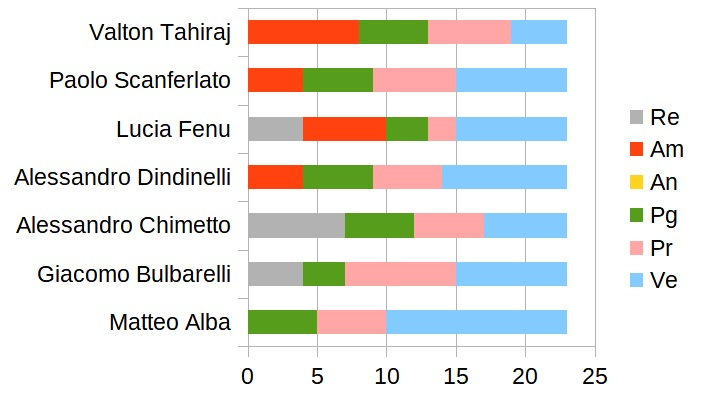
\includegraphics[width=0.8\textwidth]{res/img/grafici/validazione_e_collaudo_ore_ruolo.jpg}
			\caption{Preventivo - Validazione e collaudo - ore per persona/ruolo} 
		\end{figure}
	
	\newpage
	
	\subsubsection{Prospetto economico}
	
		\begin{table} [h!] % QUESTA RICHIEDE \usepackage{eurosym} IN config.tex
			\rowcolors{2}{gray!25}{gray!6}
			\begin{center}
				\begin{tabular} { m{3cm} >{\centering}m{1.5cm} c }
					\rowcolor{lightgray}
					\textbf{Ruolo} & \textbf{Ore} & \textbf{Costo in \euro} \\
					Responsabile & 15 & 450,00 \\
					Amministratore & 22 & 440,00 \\
					Analista & 0&0 \\
					Progettista & 31 & 682,00 \\
					Programmatore & 37 & 555,00 \\
					Verificatore & 56 & 840,00 \\
					\textbf{Totale} & \textbf{161} & \textbf{2967,00} \\
				\end{tabular}
				\caption{Preventivo - Validazione e Collaudo - costo per ruolo}
			\end{center}
		\end{table}
	
		\begin{figure} [h!]
			\centering
			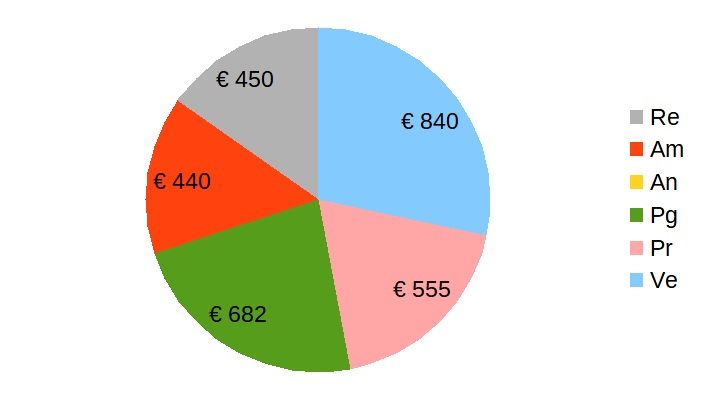
\includegraphics[width=0.8\textwidth]{res/img/grafici/validazione_e_collaudo_costi.jpg}
			\caption{Preventivo - Validazione e Collaudo - costo per ruolo} 
		\end{figure}
	
\newpage

\subsection{Riepilogo}

	\subsubsection{Prospetto orario totale di investimento}

		\begin{table} [h!]
			\rowcolors{2}{gray!25}{gray!6}
			\begin{center}
				\begin{tabular} { m{3.5cm} c c c c c c c }
					\rowcolor{lightgray}
					\textbf{Nome} & \textbf{Re} & \textbf{Am} & \textbf{An} & \textbf{Pg} & \textbf{Pr} & \textbf{Ve} & \textbf{Totale} \\
					Matteo Alba & 12 & 13 & 15 & 20 & 26& 49 & 135 \\
					Giacomo Bulbarelli & 16 & 14 & 17 & 24 & 32 & 32 & 135 \\
					Alessandro Chimetto & 18 & 11 & 21 & 24 & 23 & 38 & 135 \\
					Alessandro Dindinelli & 8 & 16 & 15 & 26 & 29 & 41 & 135 \\
					Lucia Fenu & 7 & 18 & 15 & 29 & 27 & 39 & 135 \\
					Paolo Scanferlato & 12 & 18 & 11 & 25 & 25 & 44 & 135 \\
					Valton Tahiraj & 11 & 18 & 18 & 18 & 25 & 45 & 135 \\
					\textbf{Ore totali Ruolo} & \textbf{84} & \textbf{108} & \textbf{112} & \textbf{166} & \textbf{187}& \textbf{288} & \textbf{945}
				\end{tabular}
				\caption{Preventivo - Ore totali per persona/ruolo}
			\end{center}
		\end{table}
	
		\begin{figure} [h!]
			\centering
			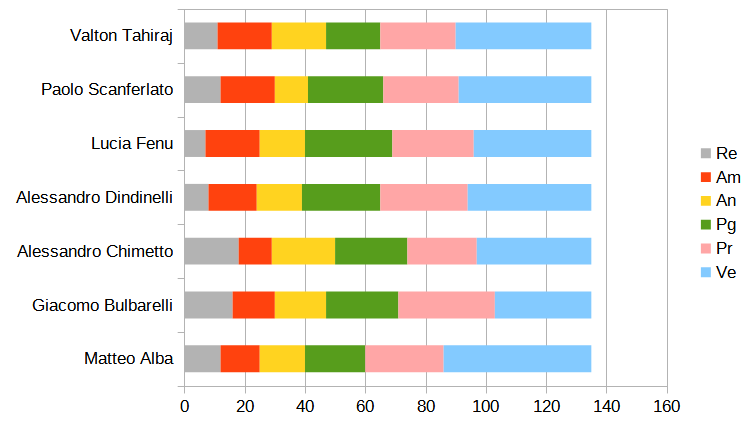
\includegraphics[width=0.8\textwidth]{res/img/preventivi/totNONrend-barre.png}
			\caption{Preventivo - Ore totali per persona/ruolo} 
		\end{figure}
	
	\newpage
	
	\subsubsection{Prospetto economico totale di investimento}
	
		\begin{table} [h!] % QUESTA RICHIEDE \usepackage{eurosym} IN config.tex
			\rowcolors{2}{gray!25}{gray!6}
			\begin{center}
				\begin{tabular} { m{3cm} >{\centering}m{1.5cm} c }
					\rowcolor{lightgray}
					\textbf{Ruolo} & \textbf{Ore} & \textbf{Costo in \euro} \\
					Responsabile & 84 & 2520,00 \\
					Amministratore & 108 & 2160,00 \\
					Analista & 112 & 2800,00 \\
					Progettista & 166 & 3652,00 \\
					Programmatore & 187 & 2805,00 \\
					Verificatore & 288 & 4320,00 \\
					\textbf{Totale} & \textbf{945} & \textbf{18257,00} \\
				\end{tabular}
				\caption{Preventivo - Costo totale per ruolo}
			\end{center}
		\end{table}
	
		\begin{figure} [h!]
			\centering
			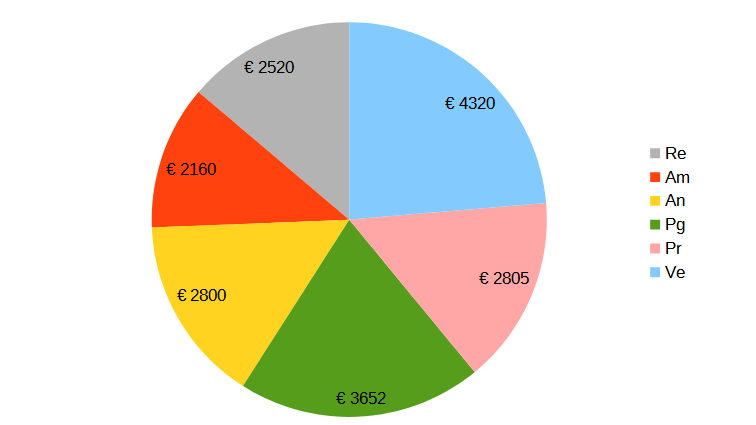
\includegraphics[width=0.8\textwidth]{res/img/preventivi/totNONrend-torta.png}
			\caption{Preventivo - Costo totale per ruolo} 
		\end{figure}
	
	\newpage
	
	\subsubsection{Prospetto orario rendicontato}

		\begin{table} [h!]
			\rowcolors{2}{gray!25}{gray!6}
			\begin{center}
				\begin{tabular} { m{3.5cm} c c c c c c c }
					\rowcolor{lightgray}
					\textbf{Nome} & \textbf{Re} & \textbf{Am} & \textbf{An} & \textbf{Pg} & \textbf{Pr} & \textbf{Ve} & \textbf{Totale} \\
					Matteo Alba & 10 & 5 & 7 & 20 & 26 & 35 & 103 \\
					Giacomo Bulbarelli & 9 & 6 & 5 & 24 & 32 & 27 & 103 \\
					Alessandro Chimetto & 11 & 6 & 9 & 24 & 23 & 30 & 103 \\
					Alessandro Dindinelli & 5 & 12 & 2 & 26 & 29 & 29 & 103 \\
					Lucia Fenu & 6 & 12 & 2 & 29 & 27 & 27 & 103 \\
					Paolo Scanferlato & 7 & 11 & 3 & 25 & 25 & 32 & 103 \\
					Valton Tahiraj & 5 & 13 & 8 & 18 & 25 & 34 & 103 \\
					\textbf{Ore totali Ruolo} & \textbf{53} & \textbf{65} & \textbf{36} & \textbf{166} & \textbf{187}& \textbf{214} & \textbf{721}
				\end{tabular}
				\caption{Preventivo - Ore totali rendicontate per persona/ruolo}
			\end{center}
		\end{table}
	
		\begin{figure} [h!]
			\centering
			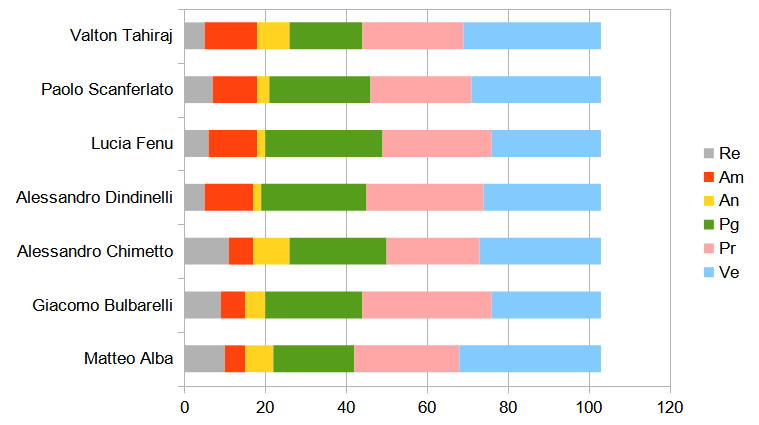
\includegraphics[width=0.8\textwidth]{res/img/preventivi/totrend-barre.png}
			\caption{Preventivo - Ore totali rendicontate per persona/ruolo} 
		\end{figure}
	
	\newpage
	
	\subsubsection{Prospetto economico rendicontato}
	
		\begin{table} [h!] % QUESTA RICHIEDE \usepackage{eurosym} IN config.tex
			\rowcolors{2}{gray!25}{gray!6}
			\begin{center}
				\begin{tabular} { m{3cm} >{\centering}m{1.5cm} c }
					\rowcolor{lightgray}
					\textbf{Ruolo} & \textbf{Ore} & \textbf{Costo in \euro} \\
					Responsabile & 53 & 1590,00 \\
					Amministratore & 65 & 1300,00 \\
					Analista & 36 & 900,00 \\
					Progettista & 166 & 3652,00 \\
					Programmatore & 187 & 2805,00 \\
					Verificatore & 214 & 3210,00 \\
					\textbf{Totale} & \textbf{721} & \textbf{13457,00} \\
				\end{tabular}
				\caption{Preventivo - Prospetto economico rendicontato per ruolo}
			\end{center}
		\end{table}
	
		\begin{figure} [h!]
			\centering
			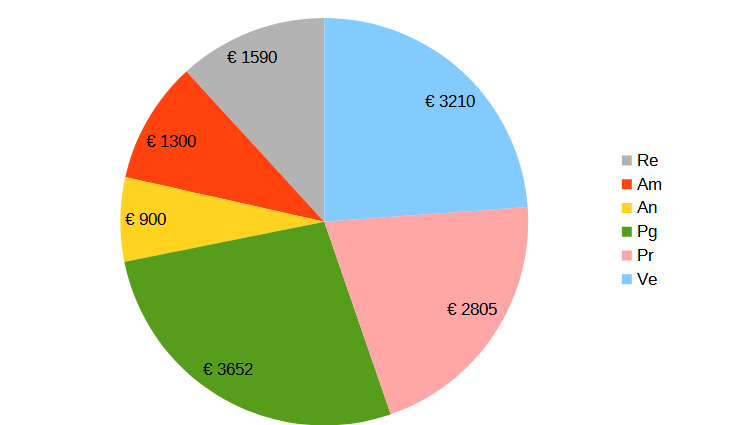
\includegraphics[width=0.8\textwidth]{res/img/preventivi/totrend-torta.png}
			\caption{Preventivo - Prospetto economico rendicontato per ruolo} 
		\end{figure}
	
	\subsubsection{Conclusioni}
	
	Il costo totale a carico della Proponente è di \textbf{\euro \ 13457,00}.
	\newpage

	\section{Consuntivo}
	
In questa sezione verrà riportato il bilancio delle ore dei vari componenti del gruppo in base ai ruoli sostenuti. Il bilancio sarà così analizzato:
\begin{itemize}
	\item {\bfseries in positivo}: se il numero delle ore effettuate è minore rispetto a quelle preventivate;
	\item {\bfseries in negativo}: se il numero delle ore effettuate è maggiore rispetto a quelle preventivate;
	\item {\bfseries in pari}: se il numero delle ore effettuate è uguale rispetto a quelle preventivate. \\
\end{itemize}

\subsection {Consuntivo di periodo: Analisi dei requisiti}
Verranno analizzate le ore di lavoro effettuate durante l'analisi dei requisiti, destinate principalmente allo studio personale; quindi non rendicontate.
\subsubsection{Prospetto orario}
	\begin{table} [h!]
	\begin{center}
		\rowcolors{2}{gray!25}{gray!6}
		\begin{tabular} { m{6 cm} c c c c c c c c }
			\rowcolor{lightgray}
			\textbf{Nome} & \textbf{Re} & \textbf{Am} & \textbf{An} & \textbf{Pg} &\textbf{Pr} & \textbf{Ve} & \textbf{Totale} \\ 
			Matteo Alba & 0 & 8(-5) &8(+4) & 0 & 0 & 10(+1) & 26  \\ 
			Giacomo Bulbarelli & 7(+4) & 6(-1) & 8(-2) & 0 & 0 & 5(-1) & 26 \\ 
			Alessandro Chimetto & 7 & 0(-4) & 11(+4) & 0 & 0 & 8 & 26 \\
			Alessandro Dindinelli & 0 & 4(-1) & 12(+1) & 0 & 0 & 10 & 26 \\
			Lucia Fenu & 0(-3) & 6(-4) & 10(+6) & 0 & 0 & 10(+1) & 26 \\
			Paolo Scanferlato & 5(+1) & 7(-4) & 6(+2) & 0 & 0 & 8(+1) & 26 \\
			Valton Tahiraj & 6(+3) & 5(-2) &7(+1) & 0 & 0 & 8(-2) & 26 \\
			\textbf{Ore Totali Ruolo} & 25(+5) & 36(-21) & 62(+16) & 0 & 0 & 59 & 182\\
		
		\end{tabular}
		\caption{Consuntivo - Analisi dei requisiti - ore per persona/ruolo}
	\end{center}
\end{table}

	\begin{figure} [h!]
	\centering
	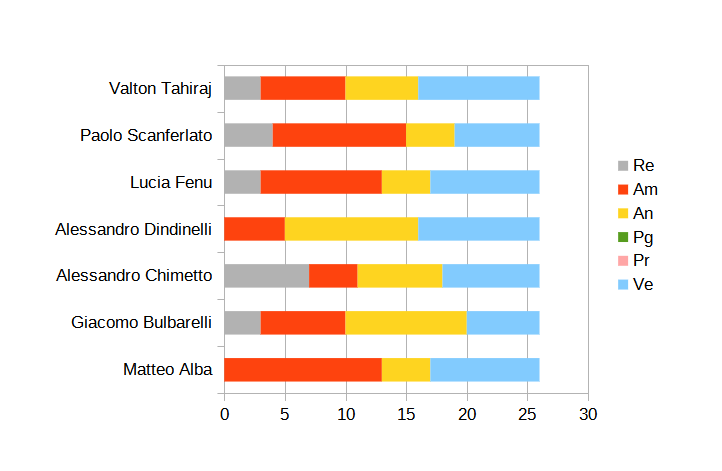
\includegraphics[width=0.7\textwidth]{res/img/grafici/consuntivo-barre_ ore analisi requisiti.png}
	\caption{Consuntivo - Analisi dei requisiti - ore di suddivisione dei ruoli} 
\end{figure}


\newpage
\subsubsection{Prospetto economico}
Nella tabella sono riportate le ore totali per ciascun costo seguendo le indicazioni descritte all'inizio della sezione.
Allo stesso modo, il costo in euro sarà così analizzato:
\begin{itemize}
	\item {\bfseries in positivo}: la somma finale è minore rispetto a quella preventivata, il proponente ha risparmiato denaro;
	\item {\bfseries in negativo}: la somma finale è maggiore rispetto a quella preventivata, il proponente ha investito più denaro;
	\item {\bfseries in pari}: la somma finale è invariata rispetto a quanto preventivato. \\
\end{itemize}
\begin{table} [h!]
	\begin{center}
		\rowcolors{2}{gray!25}{gray!6}
		\begin{tabular} { m{3 cm} c c c  }
			\rowcolor{lightgray}
			\textbf{Ruolo} & \textbf{Ore} & \textbf{Costo in \euro} \\
			Responsabile & 25(+5) & 750,00 (+150,00) \\
			Amministratore & 36(-21) & 720,00 (-420,00)  \\
			Analista & 62(+16) & 1550,00 (+400,00) \\
			Progettista & 0 & 0 \\
			Programmatore & 0 & 0  \\
			Verificatore & 59 & 885,00  \\
			\textbf{Totale} & 182  & 3905,00 (+130,00) \\
			
		\end{tabular}
		\caption{Consuntivo - Analisi dei requisiti - costo per ruolo}
	\end{center}
\end{table}

\begin{figure} [h!]
	\centering
	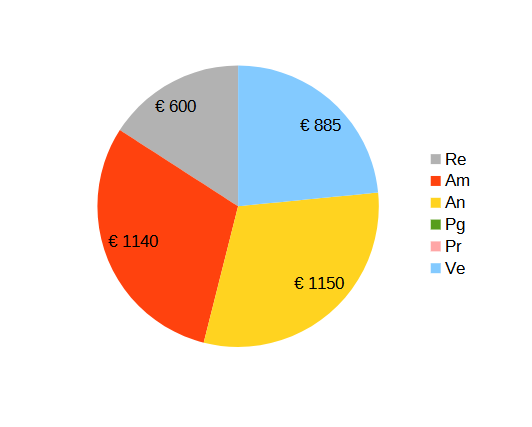
\includegraphics[width=0.6\textwidth]{res/img/grafici/consuntivo- torta_ costo_per_ora- analisi dei requisiti.png}
	\caption{Consuntivo - Analisi dei requisiti - costo per ruolo} 
\end{figure}

\newpage 

\subsubsection{Conclusioni}
Il gruppo nel complesso, ha lavorato secondo le ore preventivate seppur con alcune modifiche nella rotazione dei ruoli.
Nello specifico:
\begin{itemize}
	\item {\bfseries responsabile}: le ore previste, nel complesso, sono state rispettate. Per parallelizzare meglio il lavoro, è stato incluso un membro all'interno del ruolo (rispetto al preventivo), alleggerendo anche il carico ad altri membri;
	\item {\bfseries amministratore}: il lavoro previsto per la stesura dei documenti ha richiesto più ore rispetto a quelle preventivate, distribuite su tutti i membri;
	\item {\bfseries analista}: la stesura dell'\dext{Analisi dei requisiti} ha richiesto meno tempo rispetto a quanto preventivato e dunque, le ore mancanti, sono state distribuite nei restanti ruoli che ne necessitavano di più;
	\item {\bfseries verificatore}: grazie all'attenzione riposta nella gestione dei documenti, è stato svolto il ruolo di verificatore nelle ore previste.\\
		
	A causa della variazione oraria di alcuni ruoli, il totale prevede una spesa inferiore di \euro 130,00 rispetto a quanto preventivato.
	Tuttavia, la fase di analisi dei requisiti, non è rendicontata.
	
\end{itemize}



	

	
\newpage	
	
\subsection{Consuntivo di periodo: Analisi di dettaglio}
Verranno qui di seguito analizzate le ore per ruolo di ogni membro del gruppo sulla base del preventivo in sezione 5.2.

\subsubsection{Prospetto orario}
	\begin{table} [h!]
	\rowcolors{2}{gray!25}{gray!6}
	\begin{center}
		\begin{tabular} { m{3.5cm} c c c c c c c }
			\rowcolor{lightgray}
			\textbf{Nome} & \textbf{Re} & \textbf{Am} & \textbf{An} & \textbf{Pg} & \textbf{Pr} & \textbf{Ve} & \textbf{Totale} \\
			Matteo Alba               & 2(+2) & 0(-2) & 0      & 0  & 0  & 4      & 6 \\
			Giacomo Bulbarelli        & 0     & 2     & 4      & 0  & 0  & 0      & 6 \\
			Alessandro Chimetto       & 0(-1) & 5(+2) & 1(-1)  & 0  & 0  & 0      & 6 \\
			Alessandro Dindinelli     & 3     & 0(-2) & 1(+1)  & 0  & 0  & 2(+1)  & 6 \\
			Lucia Fenu                & 1     & 0(-2) & 3(+2)  & 0  & 0  & 2      & 6 \\
			Paolo Scanferlato         & 0     & 0     & 2      & 0  & 0  & 4      & 6 \\
			Valton Tahiraj            & 0     & 0     & 3(+1)  & 0  & 0  & 3(-1)  & 6\\
			\textbf{Ore totali Ruolo} & 6(+1) & 7(-4) & 14(+3) & 0  & 0  & 15     & 42
		\end{tabular}
		\caption{Consuntivo - Analisi di dettaglio - ore per persona/ruolo}
	\end{center}
\end{table}

	\begin{figure} [h!]
	\centering
	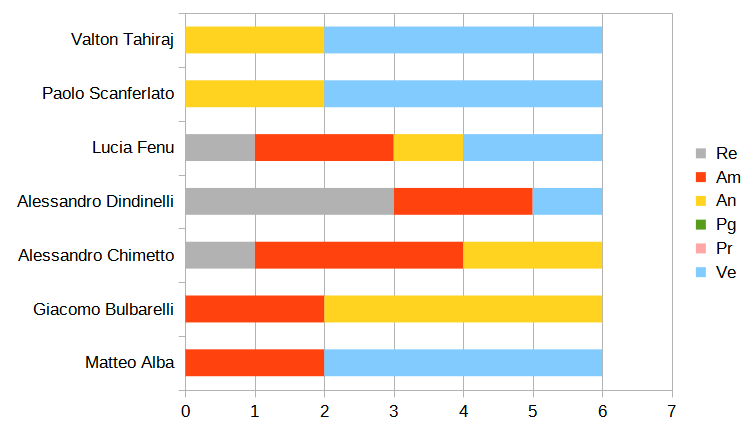
\includegraphics[width=0.7\textwidth]{res/img/grafici/consuntivo-barre- ore analisi dettaglio.png}
	\caption{Consuntivo - Analisi di dettaglio - ore di suddivisione dei ruoli} 
\end{figure}

\newpage
\subsubsection{Prospetto economico}
Nella tabella sono riportate le ore totali per ciascun costo seguendo le indicazioni descritte all'inizio della sezione.

\begin{table} [h!]
	\begin{center}
		\rowcolors{2}{gray!25}{gray!6}
		\begin{tabular} { m{3 cm} c c c  }
			\rowcolor{lightgray}
			\textbf{Ruolo}  & \textbf{Ore} & \textbf{Costo in \euro} \\
			Responsabile    & 6(+1)      & 180,00 (+30,00) \\
			Amministratore  & 7(-4)      & 140,00 (-80,00)  \\
			Analista        & 14(+3)     & 350,00 (+75,00) \\
			Progettista     & 0          & 0 \\
			Programmatore   & 0          & 0  \\
			Verificatore    & 15         & 225,00  \\
			\textbf{Totale} & 42         & 895,00 (+25,00) \\
			
		\end{tabular}
		\caption{Consuntivo - Analisi di dettaglio - costo per ruolo}
	\end{center}
\end{table}
	\begin{figure} [h!]
	\centering
	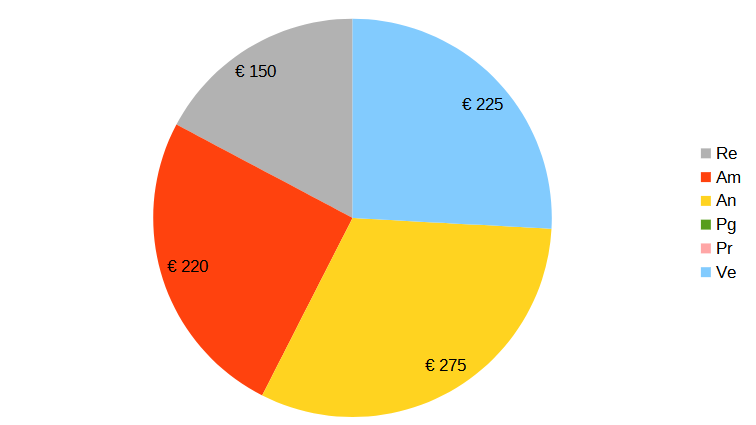
\includegraphics[width=0.7\textwidth]{res/img/grafici/consuntivo-torta-analisi di dettaglio.png}
	\caption{Consuntivo - Analisi di dettaglio - costo per ruolo} 
\end{figure}

\subsubsection{Conclusioni }
In conclusione, si osserva un risparmio orario nei ruoli di Responsabile e Analista compensato dall'investimento orario parallelo nel ruolo di Amministratore.\\
Dal punto di vista economico si osserva un leggero risparmio dei costi previsti. \\
In generale, il preventivo era corretto in un ottica generale ma non erano previsti oneri amministrativi come quelli incontrati.


\newpage

\subsection{Consuntivo di periodo: Codifica \glock{Technlogy Baseline}}
Verranno qui di seguito analizzate le ore per ruolo di ogni membro del gruppo sulla base del preventivo in sezione 5.3.
\subsubsection{Prospetto orario}
\begin{table} [h!]
	\rowcolors{2}{gray!25}{gray!6}
	\begin{center}
		\begin{tabular} { m{3.5cm} c c c c c c c }
			\rowcolor{lightgray}
			\textbf{Nome} & \textbf{Re} & \textbf{Am} & \textbf{An} & \textbf{Pg} & \textbf{Pr} & \textbf{Ve} & \textbf{Totale} \\
			Matteo Alba               & 8(+3)      & 0(-3)    & 4      & 3  & 5  & 6      & 27 \\
			Giacomo Bulbarelli        & 3     & 0     & 5(+2)  & 7  & 5(-4)  & 7(+2)      & 27 \\
			Alessandro Chimetto       & 0     & 2    & 4(+2)       & 6(-1)  & 6(-1)  & 9     & 27 \\
			Alessandro Dindinelli     & 2     & 4    & 0       & 7  & 7  & 7  & 27 \\
			Lucia Fenu                & 0(-2)  & 2(-2)  & 3      & 7(+2)   & 7(+2)   & 9      & 27 \\
			Paolo Scanferlato         & 2      & 3      & 3      & 6       & 4       & 9      & 27 \\
			Valton Tahiraj            & 0      & 3      & 4(+2)  & 3(-2)   & 6(-2)   & 11(+2) & 27\\
			\textbf{Ore totali Ruolo} & 15(+1) & 14(-5) & 23(+6) & 39(-1)  & 40(-5)  & 58(+4) & 189\\
		\end{tabular}
		\caption{Consuntivo - Codifica \glock{Technlogy Baseline} - ore per persona/ruolo}
	\end{center}
\end{table}
	\begin{figure} [h!]
	\centering
	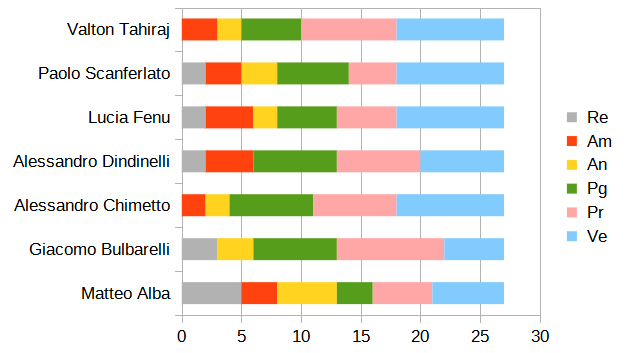
\includegraphics[width=0.7\textwidth]{res/img/grafici/consuntivo-barre-tb.png}
	\caption{Consuntivo - Codifica \glock{Technlogy Baseline} - costo per ruolo} 
\end{figure}
\newpage
\subsubsection{Prospetto economico}
Nella tabella sono riportate le ore totali per ciascun costo seguendo le indicazioni descritte all'inizio della sezione.

\begin{table} [h!]
	\begin{center}
		\rowcolors{2}{gray!25}{gray!6}
		\begin{tabular} { m{3 cm} c c c  }
			\rowcolor{lightgray}
			\textbf{Ruolo}  & \textbf{Ore} & \textbf{Costo in \euro} \\
			Responsabile    & 15(+1)      & 450,00 (+30,00) \\
			Amministratore  & 14(-5)      & 280,00 (-100,00)  \\
			Analista        & 23(+6)     & 575,00 (+150,00) \\
			Progettista     & 39(-1)          & 858,00 (-22,00) \\
			Programmatore   & 40(-5)        & 600,00 (-75,00) \\
			Verificatore    & 58(+4)        & 870,00 (+60,00) \\
			\textbf{Totale} & 189         & 3633,00 (+43,00) \\
			
		\end{tabular}
		\caption{Consuntivo - Codifica \glock{Technlogy Baseline} - costo per ruolo}
	\end{center}
\end{table}
\begin{figure} [h!]
	\centering
	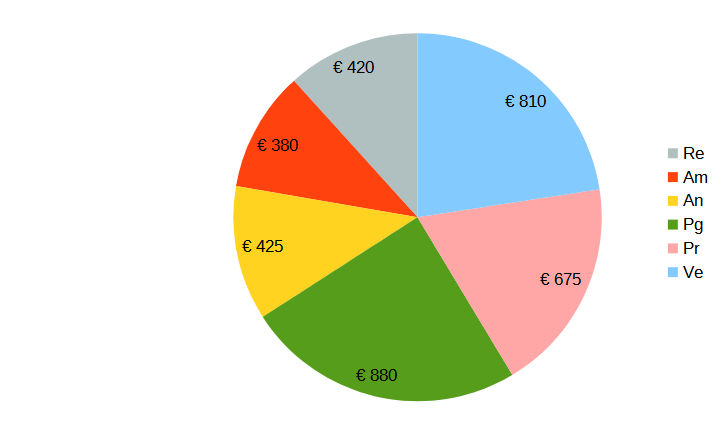
\includegraphics[width=0.7\textwidth]{res/img/grafici/consuntivo-torta-tb.png}
	\caption{Consuntivo - Codifica \glock{Technlogy Baseline} - costo per ruolo} 
\end{figure}
\subsubsection{Conclusioni}
L'impegno orario preventivato corretto rispetto al totale monte ore.\\ Decisamente meno il prospetto orario di dettaglio sui singoli ruoli: il lavoro svolto si e' incentrato molto di piu' sulla codifica e sulla progettazione, mentre (complice un workflow funzionale e una necessita' meno stringente di verificare il codice prodotto, i ruoli di Analista e Verificatore sono risultati meno importanti del previsto).\\
Il risparmio anche in questo caso e' significativo nel sottolineare come il preventivo orario sia nel corretto rispetto al monte ore finale ma da rivedere rispetto all'impegno che il singolo ruolo ha nella fase specifica di cui si fa preventivo. \\ 


	\newpage

	\appendix
	\section{Riscontro rischi}
	\begin{table} [h!]
	\rowcolors{2}{gray!25}{gray!6}
	\begin{center}
		\begin{tabular} { m{2cm} m{3cm} m{5cm} m{5cm} }
			\rowcolor{lightgray}
			\textbf{ID rischio} & \textbf{Periodo} & \textbf{Problema} & \textbf{Soluzione}\\
			RST3 & 14-12-2020 dalle ore 12.00 circa alle ore 15.30 circa & Piattaforma \glock{Google Meet} non disponibile per la riunione con il proponente a causa di guasti interni & Il team ha contattato il proponente per informarlo del disagio e i membri hanno provveduto a concordare con il proponente stesso una metodologia di incontro alternativa, poi non risultata necessaria in quanto il guasto si è risolto prima dell'orario effettivo previsto per l'incontro\\ 
			RSP1 & Per tutto il periodo antecedente la RR & Primo approccio difficoltoso alle tecnologie \glock{latex} e \glock{git} per alcuni membri del gruppo & I membri che presentavano difficoltà lo hanno reso noto al responsabile e, da egli coordinato, il gruppo ha provveduto a colmare le lacune che taluni membri presentavano \\
			RST2 & Per tutto il periodo antecedente la RR & Non sempre i membri sono stati nella condizione di poter partecipare a riunioni interne a causa di malfunzionamenti della linea internet domestica & Il gruppo provvedeva a contattare e aggiornare il membro che ha riscontrato il problema quando questi era nuovamente disponibile per comunicare \\
		\end{tabular}
	\end{center}
\end{table}
	\newpage

	\section{Organigramma}
	
\subsection{Redazione}

\begin{table} [h!]
	\begin{center}
		\renewcommand{\arraystretch}{3}
		\begin{tabular} { c c c }
			\rowcolor{lightgray}
			\textbf{Nominativo} & \textbf{Data} & \textbf{Firma} \\
			Alessandro Chimetto & 12-12-2020 & 
\includegraphics[width=0.3\textwidth]{res/img/firme/alessandro_chimetto.jpg}\\
		\end{tabular}
		\caption{Organigramma - Redazione}
	\end{center}
\end{table}


\subsection{Approvazione}

\begin{table} [h!]
	\begin{center}
		\renewcommand{\arraystretch}{3}
		\begin{tabular} { c c c }
			\rowcolor{lightgray}
			\textbf{Nominativo} & \textbf{Data} & \textbf{Firma} \\
			Paolo Scanferlato & 12-12-2020 & 
\includegraphics[width=0.2\textwidth]{res/img/firme/paolo_scanferlato.jpg}\\
			Prof. Tullio Vardanega & & \\
		\end{tabular}
		\caption{Organigramma - Approvazione}
	\end{center}
\end{table}

\newpage

\subsection{Accettazione dei componenti}
	\begin{table} [h!]
		\begin{center}
			\renewcommand{\arraystretch}{3}
			\begin{tabular} { c c c }
				\rowcolor{lightgray}
				\textbf{Nominativo} & \textbf{Data accettazione} & \textbf{Firma} \\
				Matteo Alba & 12-12-2020 & 
\includegraphics[width=0.2\textwidth]{res/img/firme/matteo_alba.jpg}\\
				Giacomo Bulbarelli & 12-12-2020 & 
\includegraphics[width=0.2\textwidth]{res/img/firme/giacomo_bulbarelli.jpg}\\
				Alessandro Chimetto & 12-12-2020 & 
\includegraphics[width=0.3\textwidth]{res/img/firme/alessandro_chimetto.jpg}\\
				Alessandro Dindinelli & 12-12-2020 & 
\includegraphics[width=0.2\textwidth]{res/img/firme/alessandro_dindinelli.jpg}\\
				Lucia Fenu & 12-12-2020 & 
\includegraphics[width=0.2\textwidth]{res/img/firme/lucia_fenu.jpg}\\
				Paolo Scanferlato & 12-12-2020 & 
\includegraphics[width=0.2\textwidth]{res/img/firme/paolo_scanferlato.jpg}\\
				Valton Tahiraj & 12-12-2020 & 
\includegraphics[width=0.2\textwidth]{res/img/firme/valton_tahiraj.jpg}\\
			\end{tabular}
			\caption{Organigramma - Accettazione dei componenti}
		\end{center}
	\end{table}

\newpage

\subsection{Componenti}
	\begin{table} [h!]
		\begin{center}
			\renewcommand{\arraystretch}{3}
			\begin{tabular} { c c c }
				\rowcolor{lightgray}
				\textbf{Nominativo} & \textbf{Matricola} & \textbf{Email} \\
				Matteo Alba & 1075682 & matteo.alba.1@studenti.unipd.it\\
				Giacomo Bulbarelli & 1144046 & giacomo.bulbarelli@studenti.unipd.it\\
				Alessandro Chimetto & 1142192 & alessandro.chimetto@studenti.unipd.it\\
				Alessandro Dindinelli & 1170457 & alessandro.dindinelli@studenti.unipd.it\\
				Lucia Fenu & 1125521 & lucia.fenu@studenti.unipd.it\\
				Paolo Scanferlato & 1170709 & paolo.scanferlato@studenti.unipd.it\\
				Valton Tahiraj & 1193389 & valton.tahiraj@studenti.unipd.it\\
			\end{tabular}
			\caption{Organigramma - Componenti}
		\end{center}
	\end{table}
	







	\newpage

\end{document}